%% Преамбула TeX-файла

% 1. Стиль и язык
\documentclass[utf8x, 14pt]{G7-32} % Стиль (по умолчанию будет 14pt)

% Остальные стандартные настройки убраны в preamble.inc.tex.
\sloppy

% Настройки стиля ГОСТ 7-32
% Для начала определяем, хотим мы или нет, чтобы рисунки и таблицы нумеровались в пределах раздела, или нам нужна сквозная нумерация.
%\EqInChapter % формулы будут нумероваться в пределах раздела
%\TableInChapter % таблицы будут нумероваться в пределах раздела
%\PicInChapter % рисунки будут нумероваться в пределах раздела

%\usepackage{titlesec}
%
%\titleformat{name=\chapter,numberless}[block]
%{\filcenter\normalsize}
%{}{1pt}{\MakeUppercase}
%
%\titleformat{\chapter}[hang]
%{\filcenter\normalsize}
%{}{1pt}{\thechapter.~\MakeUppercase}

% Добавляем гипертекстовое оглавление в PDF
\usepackage[
bookmarks=true, colorlinks=true, unicode=true,
urlcolor=black,linkcolor=black, anchorcolor=black,
citecolor=black, menucolor=black, filecolor=black,
]{hyperref}

% Изменение начертания шрифта --- после чего выглядит таймсоподобно.
% apt-get install scalable-cyrfonts-tex

\IfFileExists{cyrtimes.sty}
    {
        \usepackage{cyrtimespatched}
    }
    {
        % А если Times нету, то будет CM...
    }

\usepackage{graphicx}   % Пакет для включения рисунков

% С такими оно полями оно работает по-умолчанию:
%\RequirePackage[left=20mm,right=10mm,top=20mm,bottom=20mm,headsep=0pt]{geometry}
% Если вас тошнит от поля в 10мм --- увеличивайте до 20-ти, ну и про переплёт не забывайте:
\geometry{top=20mm}
\geometry{bottom=20mm}
\geometry{right=20mm}
\geometry{left=30mm}


% Пакет Tikz
\usepackage{tikz}
\usetikzlibrary{arrows,positioning,shadows}

% Произвольная нумерация списков.
\usepackage{enumerate}

% ячейки в несколько строчек
\usepackage{multirow}

% itemize внутри tabular
\usepackage{paralist,array}

% Центрирование подписей к плавающим окружениям
\usepackage[justification=centering]{caption}

% Нормальные шрифты
\usepackage{pscyr}

\renewcommand{\itshape}{}
\renewcommand{\bfseries}{}

\setcounter{tocdepth}{1} % задать глубину оглавления — до subsection включительно
\usepackage{lastpage}
\ifpdf
\usepackage{pdflscape} 
\else 
\usepackage{lscape} 
\fi

\usepackage{graduateWorkTitle}


%\usepackage{tocloft}
%
%\renewcommand{\cfttoctitlefont}{\hspace{0.38\textwidth} \MakeUppercase}
%\renewcommand{\cftbeforetoctitleskip}{-1em}
%%	\renewcommand{\cftaftertoctitle}{\mbox{}\hfill \\ \mbox{}\hfill{\footnotesize Стр.}\vspace{-2.5em}}
%\renewcommand{\cftchapfont}{\MakeUppercase}

	
% Настройки листингов.
\ifPDFTeX
% 8 Листинги

\usepackage{listings}

% Значения по умолчанию
\lstset{
  basicstyle= \footnotesize,
  breakatwhitespace=true,% разрыв строк только на whitespacce
  breaklines=true,       % переносить длинные строки
%   captionpos=b,          % подписи снизу -- вроде не надо
  inputencoding=cp1251,
  numbers=left,          % нумерация слева
  numberstyle=\footnotesize,
  showspaces=false,      % показывать пробелы подчеркиваниями -- идиотизм 70-х годов
  showstringspaces=false,
  showtabs=false,        % и табы тоже
  stepnumber=1,
  tabsize=4,              % кому нужны табы по 8 символов?
%  frame=single
  frame=L
}

% Стиль для псевдокода: строчки обычно короткие, поэтому размер шрифта побольше
\lstdefinestyle{pseudocode}{
  basicstyle=\small,
  keywordstyle=\color{black}\bfseries\underbar,
  language=Pseudocode,
  numberstyle=\footnotesize,
  commentstyle=\footnotesize\it
}

% Стиль для обычного кода: маленький шрифт
\lstdefinestyle{realcode}{
  basicstyle=\scriptsize,
  numberstyle=\footnotesize
}

% Стиль для коротких кусков обычного кода: средний шрифт
\lstdefinestyle{simplecode}{
  basicstyle=\footnotesize,
  numberstyle=\footnotesize
}

% Стиль для BNF
\lstdefinestyle{grammar}{
  basicstyle=\footnotesize,
  numberstyle=\footnotesize,
  stringstyle=\bfseries\ttfamily,
  language=BNF
}

% Определим свой язык для написания псевдокодов на основе Python
\lstdefinelanguage[]{Pseudocode}[]{Python}{
  morekeywords={each,empty,wait,do},% ключевые слова добавлять сюда
  morecomment=[s]{\{}{\}},% комменты {а-ля Pascal} смотрятся нагляднее
  literate=% а сюда добавлять операторы, которые хотите отображать как мат. символы
    {->}{\ensuremath{$\rightarrow$}~}2%
    {<-}{\ensuremath{$\leftarrow$}~}2%
    {:=}{\ensuremath{$\leftarrow$}~}2%
    {<--}{\ensuremath{$\Longleftarrow$}~}2%
}[keywords,comments]

% Свой язык для задания грамматик в BNF
\lstdefinelanguage[]{BNF}[]{}{
  morekeywords={},
  morecomment=[s]{@}{@},
  morestring=[b]",%
  literate=%
    {->}{\ensuremath{$\rightarrow$}~}2%
    {*}{\ensuremath{$^*$}~}2%
    {+}{\ensuremath{$^+$}~}2%
    {|}{\ensuremath{$|$}~}2%
}[keywords,comments,strings]

% Подписи к листингам на русском языке.
\renewcommand\lstlistingname{\cyr\CYRL\cyri\cyrs\cyrt\cyri\cyrn\cyrg}
\renewcommand\lstlistlistingname{\cyr\CYRL\cyri\cyrs\cyrt\cyri\cyrn\cyrg\cyri}

\else
\usepackage{local-minted}
\fi

\usepackage{pdfpages}

% Полезные макросы листингов.
% Любимые команды
\newcommand{\Code}[1]{\textbf{#1}}


% Автоподсчет количества рисунков, таблиц, источников, приложений, частей.
\newcounter{totfigures}
\newcounter{tottables}
\newcounter{totalltables}
\newcounter{totreferences}
\newcounter{totappendix}
\newcounter{totchapters}
\newcounter{totallchapters}

\usepackage{etoolbox}
\makeatletter
\newif\ifLT@nocaption
\preto\longtable{\LT@nocaptiontrue}
\appto\endlongtable{%
	\ifLT@nocaption
	\addtocounter{table}{\m@ne}%
	\fi}
\preto\LT@caption{%
	\noalign{\global\LT@nocaptionfalse}}
\makeatother

\makeatletter
\AtEndDocument{%
	\immediate\write\@mainaux{%
		\string\gdef\string\totfig{\number\value{totfigures}}%
		\string\gdef\string\tottab{\number\value{tottables}}%   
		\string\gdef\string\totbib{\number\value{totreferences}}%  
		\string\gdef\string\totappend{\number\value{totappendix}}% 
		\string\gdef\string\totchaps{\number\value{totchapters}}
	}%
}
\makeatother

\usepackage{etoolbox}
\appto{\endfigure}{\addtocounter{totfigures}{1}}{}{}
\appto{\endtable}{\addtocounter{totalltables}{1}}{}{}
\appto{\endlongtable}{\addtocounter{totalltables}{1}}{}{}
\pretocmd{\bibitem}{\addtocounter{totreferences}{1}}{}{}
\pretocmd{\chapter}{\addtocounter{totappendix}{1}}{}{}
\pretocmd{\appendix}{\setcounter{totappendix}{0}}{}{}

\pretocmd{\chapter}{\addtocounter{totallchapters}{1}}{}{}
\pretocmd{\mainmatter}{\setcounter{totallchapters}{0}}{}{}	\pretocmd{\backmatter}{\setcounter{totchapters}{\thetotallchapters}}{}{}
\pretocmd{\appendix}{\setcounter{tottables}{\thetotalltables}}{}{}

\begin{document}
	
	\title{Разработка ПО для автоматизации конфигурирования сетевого оборудования CISCO}
	\subtitle{Выпускная квалификационная работа\\
		Пояснительная записка\\
		090301 000 000 314 ПЗ}
	\teachers{1}{Трофимов С.П.}
	\students{1}{Черетаев И.В.}
	\controllers{1}{Селиванова И.А.}
	\group{РИ-420207}
	\city{Екатеринбург}
	\thispagestyle{empty}
	
\includepdf[pages=-,pagecommand={}]{titul}
%	\maketitle
%	\setcounter{page}{2} % начать нумерацию страниц с №2
	
\frontmatter % выключает нумерацию ВСЕГО; здесь начинаются ненумерованные главы: реферат, введение, глоссарий, сокращения и прочее.

% Команды \breakingbeforechapters и \nonbreakingbeforechapters
% управляют разрывом страницы перед главами.
% По-умолчанию страница разрывается.

% \nobreakingbeforechapters
% \breakingbeforechapters


% Также можно использовать \Referat, как в оригинале

%\begin{abstract}
	
	\chapter*{РЕФЕРАТ}
	\addcontentsline{toc}{chapter}{РЕФЕРАТ}
	
	Пояснительная записка \begin{NoHyper}{\pageref{LastPage}}\end{NoHyper}~с., 
%	\totchaps~ч., 
	\totfig~рис., \tottab~табл., \totbib~источников.%, \totappend~прил.
	
	 
	
	СЕТЕВОЕ ОБОРУДОВАНИЕ, КОНФИГУРАЦИОННЫЕ ФАЙЛЫ, МАРШРУТИЗАТОРЫ, КОММУТАТОРЫ, CISCO IOS, DHCP, NAT, VLAN, СПИСКИ ДОСТУПА.
	
	Объектом исследования выступает сетевое оборудование компании Cisco Systems
	
	Предметом исследования в дипломной работе являются настройка сетевого оборудование Cisco Systems.
	
	Теоретическая значимость дипломного исследования состоит в развитии и совершенствовании методологии настройки оборудования информационной инфраструктуры предприятия.
	
	Практическая значимость работы определяется тем, что ее результаты позволяют повысить степень эффективности настройки информационной инфраструктуры предприятия и снизить связанные с этим операционные расходы при использовании разработанной системы, направленной на повышение уровня таких аспектов администрирование, как быстрота и легкость обслуживания.
	
	Новизна дипломной работы заключается в разработке и реализации кроссплатформенной модели автоматизации конфигурирования оборудования.
%\end{abstract}

%%% Local Variables: 
%%% mode: latex
%%% TeX-master: "rpz"
%%% End: 
  

%\linespread{1.45}
\tableofcontents
%\linespread{1.5}
%\linespread{\Gost@LineSpread}

\chapter*{НОРМАТИВНЫЕ ССЫЛКИ}
\addcontentsline{toc}{chapter}{НОРМАТИВНЫЕ ССЫЛКИ}

В пояснительной записке использованы ссылки на следующие стандарты:

\begin{table*}
	\begin{tabular}{p{0.35\textwidth}p{0.65\textwidth}}
		ГОСТ 34.602-89 & Информационная технология. Комплекс стандартов на автоматизированные системы. Техническое задание на создание автоматизированной системы.\\	
		
		
		ГОСТ 7.32-2001 &	Система стандартов по информации, библиотечному и издательскому делу. Отчет о научно-исследовательской работе. Структура и правила оформления.\\
		
		ISO/IEC 12207:2008 (ГОСТ~Р). & Системная и программная инженерия. Процессы жизненного цикла программных средств.\\
		
		Cisco IOS Con\-figuration Fundamentals Command Reference & Список команд настройки Cisco IOS\\
		
	\end{tabular}
	\label{tab:tabular}
\end{table*}
%%\Defines % Необходимые определения. Вряд ли понадобться
%\begin{description}
%\item[Распределённый] Слово, которое нельзя употреблять. Но надо протестировать длинные строки в глоссарии.
%\end{description}

\chapter*{ОПРЕДЕЛЕНИЯ}

\begin{table*}
	\begin{tabular}{p{0.25\textwidth}p{0.75\textwidth}}
		Маршрутизатор & Специализированный сетевой компьютер, имеющий два или более сетевых интерфейсов и пересылающий пакеты данных между различными сегментами сети \\
	
		Коммутатор & Устройство, предназначенное для соединения нескольких узлов компьютерной сети в пределах одного сегмента сети\\
	
		
	\end{tabular}
	\label{tab:tabular}
\end{table*}




%%% Local Variables:
%%% mode: latex
%%% TeX-master: "rpz"
%%% End:

\chapter*{ОПРЕДЕЛЕНИЯ, ОБОЗНАЧЕНИЯ И СОКРАЩЕНИЯ}
\addcontentsline{toc}{chapter}{ОПРЕДЕЛЕНИЯ, ОБОЗНАЧЕНИЯ И СОКРАЩЕНИЯ}

\makeatletter
\setlength{\@fptop}{0pt}
\makeatother

\begin{table*}[ht!]
	\begin{tabular}{p{0.22\textwidth}p{0.78\textwidth}}
%		\label{tab:tabular}
		Маршрутизатор & Специализированный сетевой компьютер, имеющий два или более сетевых интерфейсов и пересылающий пакеты данных между различными сегментами сети \\
		
		Коммутатор & Устройство, предназначенное для соединения нескольких узлов компьютерной сети в пределах одного сегмента сети\\

		ПО & Программное обеспечение\\
		
		Cisco IOS & Internetwork Operating System — Межсетевая Операционная Система --- программное обеспечение, используемое в маршрутизаторах и сетевых коммутаторах Cisco\\
		
		VLAN & Virtual Local Area Network --- группа устройств, имеющих возможность взаимодействовать между собой напрямую на канальном уровне, хотя физически при этом они могут быть подключены к разным сетевым коммутаторам\\
		
		IDE & Integrated development environment --- комплекс программных средств, используемый программистами для разработки программного обеспечения\\
		
		TCP/IP & Transmission Control Protocol / Internet Protocol --- набор сетевых протоколов передачи данных, используемых в сетях, включая сеть Интернет\\
		
		IP &  Internet Protocol --- маршрутизируемый протокол сетевого уровня стека TCP/IP\\
		
		DHCP & Dynamic Host Configuration Protocol --- это сетевой протокол, позволяющий компьютерам автоматически получать IP-адрес\\
		
		
		
	\end{tabular}
	
\end{table*}

\makeatletter
\setlength{\@fptop}{0pt}
\makeatother

\begin{table*}[ht!]
	\begin{tabular}{p{0.22\textwidth}p{0.78\textwidth}}
		
		OSPF & Open Shortest Path First --- протокол динамической маршрутизации, основанный на технологии отслеживания состояния канала и использующий для нахождения кратчайшего пути алгоритм Дейкстры.\\
		
		
		EIGRP & Enhanced Interior Gateway Routing Protocol --- проприетарный протокол динамической маршрутизации класса "вектор расстояния" (Distance Vector), в котором информация передается от соседа к соседу, каждый следующий выбирает только лучший маршрут, отдаваемый соседу.\\	
		
		NAT &  Network Address Translation --- механизм в сетях TCP/IP, позволяющий преобразовывать IP-адреса транзитных пакетов\\
		
		ACL & Access Control List --- список правил, определяющих порты служб или имена доменов, доступных на узле или другом устройстве\\
		
		
		
			
	\end{tabular}	
\end{table*}
		
%%% Local Variables:
%%% mode: latex
%%% TeX-master: "rpz"
%%% End:


\Introduction

Во второй половине прошлого века в связи с «рождением» первых
вычислительных сетей произошла очередная научно-техническая революция. Появилась возможность начать использование рассредоточенной
обработки данных, обширно использовать для автоматизации различных
видов деятельности новые технологии. 



В наше время происходит активное применение сетевых решений во многих сферах деятельности. В условиях производства, на различных предприятиях,
в офисах компаний, различных фирмах и учреждениях отдельно стоящий, не подключенный к сети компьютер является большой редкостью. Если же подобной сети в учреждении нет или она плохо развита, от системных администраторов данной организации либо от специалистов компании, предоставляющей услуги в области сетевых технологий, требуется спроектировать и настроить сеть, удовлетворяющую потребностям клиента.

Важным моментом при этом является настройка сетевого оборудования. Одним из представителей компаний-производителей сетевого оборудования является Cisco Systems. Cisco Systems — компания-производитель
сетевого оборудования, основанная в 1984. Сначала компания производила маршрутизаторы, но затем значительно расширила ассортимент своей продукции. В настоящее время она производит коммутаторы, маршрутизаторы,
IP-телефоны, программное обеспечение для своего оборудования.



Специалистам, настраивающим оборудование Cisco, часто приходится использовать однообразные наборы команд конфигурации, порой отличающимися небольшим набором параметров, такими как IP-адрес устройства, идентификатор VLAN или диапазон IP-адресов при настройка DHCP.

% --- комплекс действий, для которых необходимо качество и точность выполнения. И, одновременно с этим, за прошедшее время настройка оборудования превратилась в 

Соответственно, необходимо решение, которое поможет быстро и легко настроить оборудование Cisco путем создания конфигурационных файлов для данного оборудования на основании различных шаблонов и введенных пользователем данных.

\mainmatter % это включает нумерацию глав и секций в документе ниже

	\chapter{ЗАДАЧА АВТОМАТИЗАЦИИ КОНФИГУРИРОВАНИЯ СЕТЕВОГО ОБОРУДОВАНИЯ}
	
	Специалистам, настраивающим оборудование Cisco, часто приходится использовать однообразные наборы команд конфигурации, порой отличающимися небольшим набором параметров, такими как IP-адрес устройства, идентификатор VLAN или диапазон IP-адресов при настройка DHCP.
	
	В связи с этим возникает задача автоматизировать процесс получения набора команд конфигурации, обеспечивающих следующий функционал:
	
	\begin{itemize}
		\item начальная настройка оборудования;
		\item настройка интерфейсов коммутатора/маршрутизатора;
		\item настройка VLAN'ов на коммутаторах;
		\item настройка DHCP на маршрутизаторах;
		\item настройка NAT на маршрутизаторах;
		\item настройка ACL(обычные и расширенные) на маршрутизаторах.
	\end{itemize}
	
	К программному обеспечению, решающему данную задачу, так же можно предъявить несколько требований:
	
	\begin{itemize}
		\item бесплатность;
		\item кроссплатформенность.
	\end{itemize} 
	
	Рассмотрим несколько приложений, позволяющих решить данную задачу.
%	
%	Сначала несколько слов по терминологии.
%	
%	Симуляторы — реализуют статичное множество команд, но, только
%	пользователь выходит за рамки возможного, выдают сообщение об ошибке. Классическим примером является Cisco Packet Tracer.
%	
%	Эмуляторы — дают возможность выполнять команды образов настоящих устройств, порой без заметных урезаний функциональности. Эмулятором, к примеру, является GNS3/Dynamips.
	
	\section{Cisco Packet Tracer}
	
	Packet Tracet  –-- официально выпускаемое Cisco
	программное обеспечение. Данный продукт доступен в версиях как для
	Windows, так и для Linux, бесплатно для учащихся Сетевой Академии
	Cisco.
	
	Интерфейс программы представлен на рисунке \ref{fig:packet_tracer}. Вся настройка осуществляется при помощи логической диаграммы сети.
	
	\begin{figure}[h!]
		\centering
		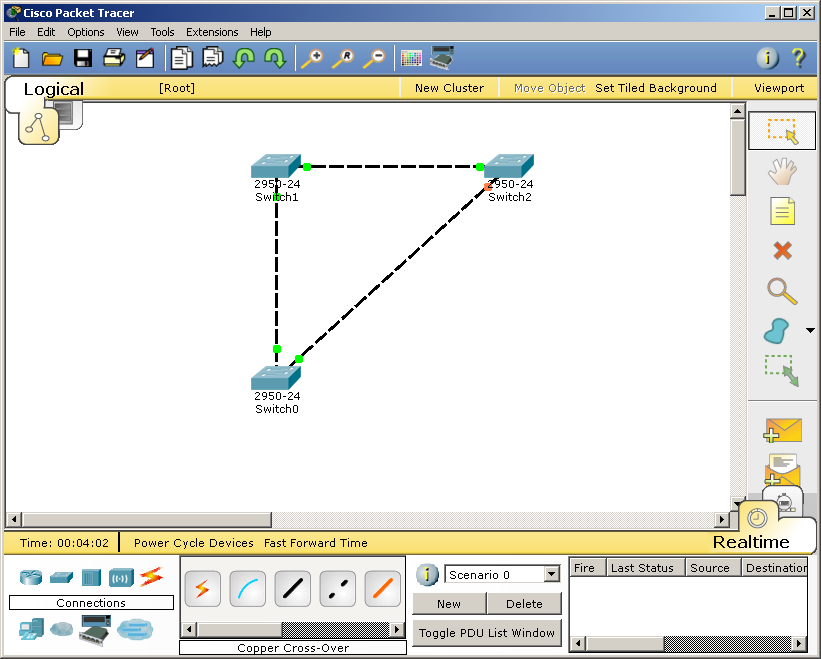
\includegraphics[width=0.9\linewidth]{pic/packet_tracer}
		\caption{Cisco Packet Tracer}
		\label{fig:packet_tracer}
	\end{figure}
	
	Достоинства Packet Tracer:
	
	\begin{itemize}
		\item дружественность и логичность интерфейса;
		\item доступность большого набора оборудования, выпускаемого Cisco;
		\item возможность перейти в режим симуляции и увидеть все действия с пакетами с использованием замедления времени.
	\end{itemize}
	
	Однако, поскольку Packet Tracer имитирует поведение оборудования Cisco, большинство действий по настройке производятся путем ввода необходимых команд в командную строку устройства, так же как если пользователь взаимодействовал бы с реальным оборудование.
	
	\section{GNS3}
	
	
	GNS3 (Graphical Network Simulator) --- представляет собой графический интерфейс, написанный на Qt, для эмулятора dynamips.
	
	Интерфейс программы продемонстрирован на рисунке \ref{fig:gns3}.
	GNS3 является свободно распространяемым проектом и доступен под следующими операционными системами: Linux, Windows и Mac OS X.
		
	\begin{figure}[h!]
		\centering
		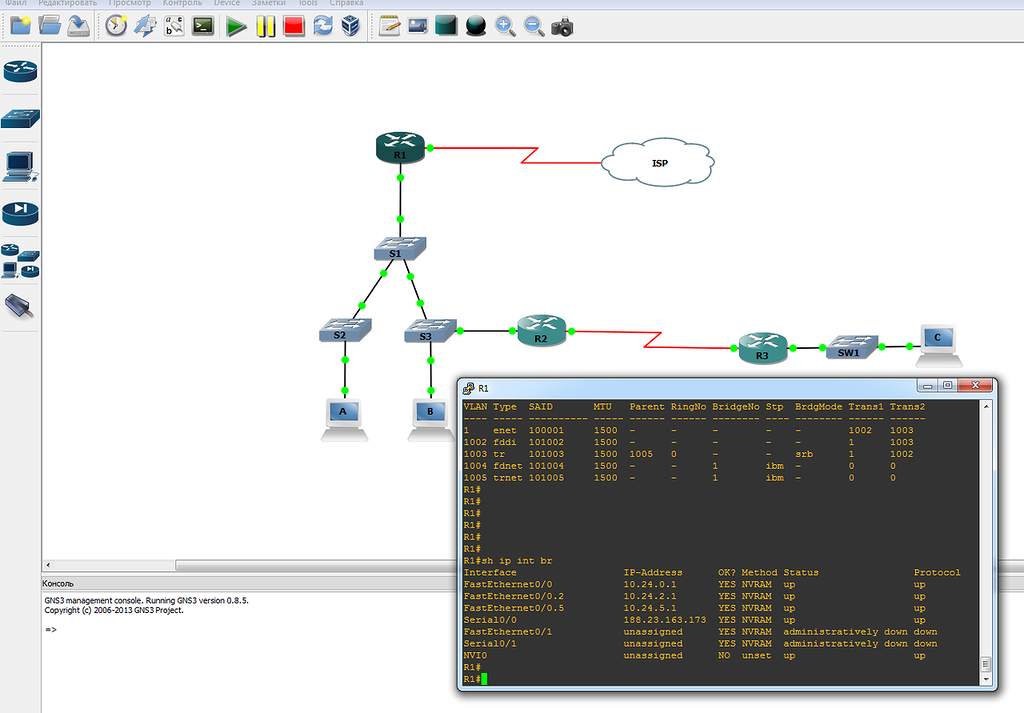
\includegraphics[width=0.9\linewidth]{pic/gns3}
		\caption{GNS3}
		\label{fig:gns3}
	\end{figure}
	
	GNS3 является эмулятором, который работает с оригинальными прошивками IOS.
	Это означает, что для использования GNS3, необходимо иметь в наличии реальные образы.
	
	Так же имеется ряд других недостатков:
	\begin{itemize}
		\item невозможность полноценно использовать коммутаторы;
		\item высокие требования к системным ресурсам;
		\item уменьшение производительности при увеличении количества устройств.
	\end{itemize}
		
	\section{Boson NetSim}
	
	Доступен в версии только для Windows, цена колеблется от 179\$ за CCNA и до 349\$ за CCNP.
	
	Выступает в роли набора лабораторных работ, объединенных по темам экзамена. Интерфейс разделен на нескольких разделов: постановка задачи, карта сети, в
	левой части находится список доступных лабораторных работ (в соответствии с рисунком \ref{fig:netsim}).
	
	После завершении выполнения лабораторной работы, можно получить результат и узнать, все ли было
	сделано.
	
	Присутствует возможность создания собственных топологий, с некоторыми
	ограничениями.
	
	
	\begin{figure}[h!]
		\centering
		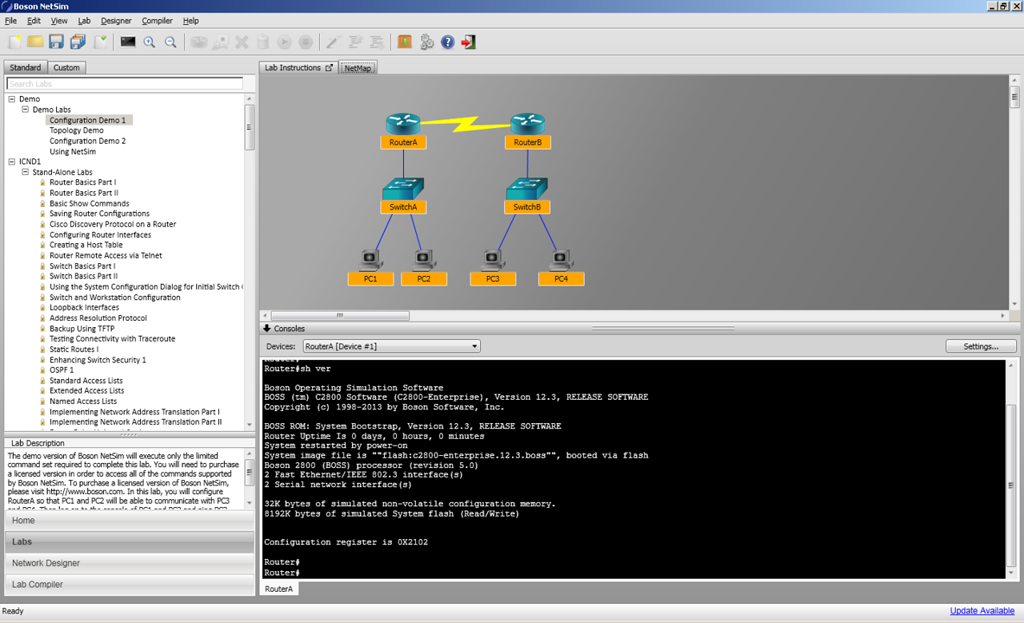
\includegraphics[width=0.9\linewidth]{pic/netsim}
		\caption{Boson NetSim}
		\label{fig:netsim}
	\end{figure}
	
	Ключевые возможности Boson NetSim:
	
	\begin{itemize}
		\item поддержка  42 маршрутизаторов, 6 коммутаторов;
		\item симуляция сетевого трафика при помощи технологии виртуальных
		пакетов;
		\item два режима просмотра: telnet или подключение по консоли;
		\item возможность создания собственных лабораторий.
	\end{itemize}
	
	\section{Cisco IOU}
	
	Последний в этом списке это  Cisco IOU (Cisco IOS on UNIX) —
	проприетарное ПО, которое официально не распространяется.
	
	Интерфейс программы представлен на рисунке \ref*{fig:ciscoIOU}.
	
	\begin{figure}[h!]
		\centering
		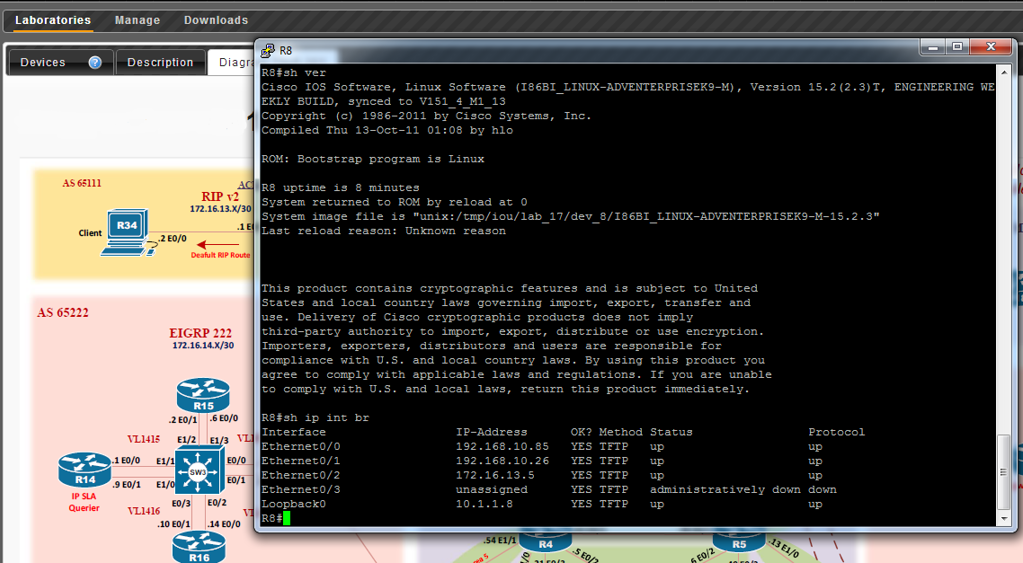
\includegraphics[width=0.9\linewidth]{pic/ciscoIOU}
		\caption{Cisco IOU}
		\label{fig:ciscoIOU}
	\end{figure}
	
	Существует мнение, что у Cisco есть возможность отследить и идентифицировать того, кто использует IOU.
	Известный факт состоит в том, что центр технической поддержки Cisco использует именно данных продукт.
	
	Сначала  был доступен только под Solaris, но затем был портирован и
	на Linux. В комплекте идут две основные части --- l2iou и l3iou. Первая часть эмулирует канальный уровень и коммутаторы, вторая же — сетевой уровень и маршрутизаторы.
	
	Настройка проводится путем редактирования конфигурационных файлов.%, недавно для него стал доступен также графический интерфейс.
	
%	Интерфейс довольно интуитивен, и позволяет выполнять почти все действия.
%	
%	В тоже время, включение на моделирование топологии, указанной на рис. \ref{fig:topologyCCIE}, приводит примерно к 50\% 	загрузке процессора.
%	
%	\begin{figure}[h!]
%		\centering
%		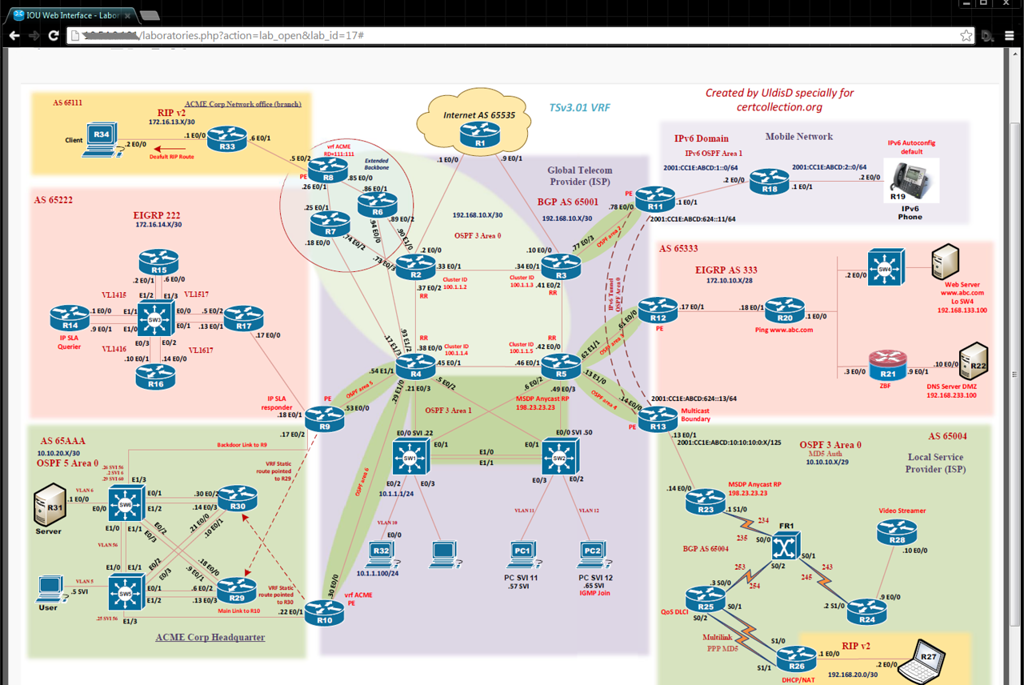
\includegraphics[width=0.7\linewidth]{pic/topologyCCIE}
%		\caption{Пример топологии}
%		\label{fig:topologyCCIE}
%	\end{figure}
%	
%	Надо сказать, данная топология предназначена для подготовки к сдаче экзамена на Cisco Certified Internetwork Expert.
%	
%	Возможности IOU на самом деле очень широкие. В тоже время, некоторые проблемы на канальном уровне все же имеются. Для некоторых устройств, например, отсутствует возможность жестко выставить дуплексный режим, но это всё мелочи.

	
	Сравнение рассмотренных программных продуктов приведено в таблице \ref{tab:econ_effect}.
	
	Общим недостатком представленных программных продуктов можно назвать излишнюю комплексность решения, вызванную попытками смоделировать полное поведение сетевых технологий. Это, в свою очередь, приводит к тому, графический интерфейс данных программ дает возможность пользователю построить логическую схему сети, но почти вся дальнейшая настройка, исключая, к примеру, название оборудования, производится путем ручного ввода соответствующих команд. И, как следствие,  отсутствует возможность шаблонизировать настройку требуемого функционала для дальнейшего использования на реальных устройствах.
	
	\begin{landscape}
		\begin{longtable}{|p{3.5cm}|p{5cm}|p{5cm}|p{5cm}|p{5cm}|} 
		% Вертикальная черта означает, что между полями должна быть вертикальная черта - разделитель
		% Заголовок таблицы на первой странице:
		\caption{Сравнение существующих решений\label{tab:econ_effect}}\\
		\hline % Вставляем горизонтальную линию
		{\centering Наименование показателей} & \centering Cisco Packet Tracer & \centering GNS3  & \centering Boson NetSim & Cisco IOU \\
		\hline
		\endfirsthead % Всё, что расположено выше считается заголовком таблицы и отображается на первой странице
		% Для второй и последующих страниц подменяем наименование таблицы в соответствии с требованиями:
		\caption*{Продолжение таблицы \ref{tab:econ_effect}}\\
		\hline
		\centering 1 & \centering 2 & \centering 3 \\
		\endhead % Всё что выше будет вставляться как заголовок на 2 и последующих страницах
		\hline
		
		Тип решения & симулятор & эмулятор & симулятор & симулятор \\
		\hline
		Ценовая политика & доступен студентам сетевой академии Cisco & бесплатен & от 179\$ за CCNA и до 349\$ за CCNP & проприетарен \\
		\hline
		Версии ОС & Windows, Linux & Linux, Windows и Mac OS X & Windows & Solaris, Linux \\

		\hline
	\end{longtable}
	
	
	
	\end{landscape}
\chapter{ВЫБОР ИНСТРУМЕНТАЛЬНОЙ СИСТЕМЫ РАЗРАБОТКИ ПО}
	
	В ходе подготовки к написанию выпускной квалификационной работы были рассмотрены несколько инструментальных сред разработки на C/C++. В качестве критериев для выбора IDE были выбраны следующие:
	
	\begin{itemize}
		\item IDE должна поддерживать разработку графического интерфейса пользователя;
		\item кроссплатформанная разработка;
		\item удобство программирования.
	\end{itemize}
	
	\section{Code::Blocks}
	
	Свободная кроссплатформенная среда разработки. 
	
	Для разработки графического интерфейса необходимо использовать плагин wxSmith, который, по сути, является  wxWidgets
	RAD инструментом, то есть позволяет создавать оконные формы и прочие графические объекты, используя библиотеку wxWidgets (библиотека wxWidgets устанавливается отдельно). 
	
	Плюсы Code::Blocks:
	
	 \begin{itemize}
		 \item автозавершение кода;
		 \item просмотрщик классов;
		 \item быстрая система сборки (не требуются make-файлы);
		 \item поддержка параллельных сборок.
	 \end{itemize}
	 
	\section{Microsoft Visual Studio Express}
	
	
	Данная версия Visual Studio представляет собой набор урезанных средств
	разработки для языков Visual Basic, C\# и C++, и обозначается Microsoft как инструментальная среда разработки начального
	уровня для тех лиц, кто не занимается профессионально программированием
	(школьников, студентов, любителей и т.д.).
	
	Графический интерфейс и возможность создать оконные приложения присутствует, но возможность воспользоваться наработками компании в области оптимизации и рефакторинга кода почти отсутствует.
	
	\section{Qt Creator}
	
	Qt Creator является средой разработки для кроссплатформенного фреймворка Qt. Вследствие этого, нужно указать на следующие его возможности:
	\begin{itemize}
		\item интеграция дизайнера форм Qt и справочной системы Qt
		\item расширяемость (посредством плагинов)
		\item поддержка отладчиков GDB (отладка графический интерфейса) и CDB
	\end{itemize}
	
	Общее сравнение IDE приведено в таблице \ref{tab:ide_effect}.
	
	\begin{longtable}{|p{3.5cm}|p{3.5cm}|p{4cm}|p{3.5cm}|}
		% Вертикальная черта означает, что между полями должна быть вертикальная черта - разделитель
		% Заголовок таблицы на первой странице:
		\caption{Сравнение IDE\label{tab:ide_effect}}\\
		\hline % Вставляем горизонтальную линию
	Наименование показателей & Code::Blocks & Microsoft Visual Studio Express & Qt Creator \\
		\hline
		\endfirsthead % Всё, что расположено выше считается заголовком таблицы и отображается на первой странице
		% Для второй и последующих страниц подменяем наименование таблицы в соответствии с требованиями:
		\caption*{Продолжение таблицы \ref{tab:ide_effect}}\\
		\hline
		\multicolumn{1}{|c|}{1} & \multicolumn{1}{|c|}{2 } & \multicolumn{1}{|c|}{3} & \multicolumn{1}{|c|}{4}\\
		\endhead % Всё что выше будет вставляться как заголовок на 2 и последующих страницах
		\hline
		
		Лицензия & \multicolumn{1}{c|}{GPL} & \multicolumn{1}{c|}{Freeware} & \multicolumn{1}{c|}{GPL} \\
		\hline
		Кроссплат\-форменность & \multicolumn{1}{c|}{Да} & \multicolumn{1}{c|}{Нет} & \multicolumn{1}{c|}{Да}  \\
		\hline
		Разработка GUI & \multicolumn{1}{c|}{Да\footnote{С использованием плагина wxSmith}} & \multicolumn{1}{c|}{Да} & \multicolumn{1}{c|}{Да} \\
		
		\hline
	\end{longtable}
	
	
	Исходя из приведенных выше сведений, было принято решение, что приложение будет написано в среде Qt Creator с использованием кроссплатформенного фреймворка Qt на языке C++. Это позволит сократить время на разработку, избежать написания большого количества кода, посредством использования готовых библиотек. Использование библиотеки Qt также поможет создать удобный интерфейс, отличный от стандартного.
	\chapter{ТЕХНИЧЕСКОЕ ЗАДАНИЕ}
	
	\section{Общие сведения}
	
	\subsection{Полное наименование системы и ее условное обозначение}
	
	Программное обеспечение для автоматизации конфигурирования сетевого оборудования Cisco. Условное обозначение – АКСО\cite{gost-34602}.
	
	\subsection{Краткая характеристика области применения}
	
	АКСО предназначено для автоматизации конфигурирования сетевого оборудования Cisco путем предоставления пользователю графического интерфейса с последующим получением набора команд, необходимых для внедрения изменений внесенных пользователем.
	
	\subsection{Перечень документов, на основании которых создается система}
	
	\begin{enumerate}
		\item Приказ ректора УрФУ № \_\_\_\_\_\_ от "\_\_\_"\_\_\_\_\_\_\_\_\_\_ \_\_\_\_\_г.
	\end{enumerate}
		
	\subsection{Перечень документов, на основании которых устанавливается порядок оформления и предъявления результатов работ}
	
	\begin{enumerate}
		\item ГОСТ 7.32-2001. Система стандартов по информации, библиотечному и издательскому делу. Отчет о научно-исследовательской работе. Структура и правила оформления\cite{gost-732}.
%		\item ГОСТ 34.602-89 Информационная технология. Комплекс стандартов на автоматизированные системы. Техническое задание на создание автоматизированной системы.
%		\item оформление ВКР !!!!!
%		\item  Методические указания по выполнению выпускной квалификационной работы бакалавра техники и технологий по направлению "Информатика и вычислительная техника" / сост. А.Б.Николаев. – Москва: МАДИ, 2010. – 17 с.
		\item Соколов С.С. Рекомендации по оформлению курсовых, выпускных и дипломных проектов (работ). Электронные методические указания - Екатеринбург: Изд. УрФУ, 2010. - 38 с.
	\end{enumerate}
	
	
	\section{Назначение разработки}
	
	\subsection{Функциональное назначение}
	
	Функциональным назначением АКСО является предоставлению пользователю удобных инструментов для облегчения конфигурирования сетевого оборудования от компании Cisco Systems, таких как маршрутизаторы и/или коммутаторы.
	
	\subsection{Эксплуатационное назначение}
	
	АКСО предназначено для автоматизации процесса конфигурирования сетевого оборудования с целью получения исходного текста конфигурации либо автоматического применения внесенных с помощью АКСО изменений на сетевом оборудовании.
	
	\section{Требования к программному средству}
	
	\subsection{Требования к функциям, выполняемым системой }
	
	\begin{enumerate}
%		\item Разработать структуру классов, хранящую информацию о сетевых устройствах.
		
%		\item Наличие основных моделей маршрутизаторов и коммутаторов.
		
		\item Программа должна обеспечивать генерацию команд конфигурации, обеспечивающих:
		\begin{itemize}
			\item начальную настройку оборудования;
			\item настройку интерфейсов коммутатора/маршрутизатора;
			\item настройку VLAN'ов на коммутаторах;
			\item настройку DHCP на маршрутизаторах;
			\item настройку NAT на маршрутизаторах;
			\item настройку ACL(обычные и расширенные) на маршрутизаторах.
		\end{itemize}
		
		\item Наличие редактора, позволяющего добавлять и редактировать шаблоны.  Редактор должен обеспечивать возможность поиска в списке имеющихся моделей. 
%		Так же при помощи данного редактора должны производиться операции визуального изменения конфигурации для выбранного модели сетевого оборудования.

		\item Возможность выбора шаблона и ввода необходимых параметров в шаблон.		
		
%		\item Наличие возможности экпорта/импорта выбранной конфигурации в виде XML-файла, содержащего все необходимые сведения.
		
		\item Наличие возможности сохранения сгенерированной конфигурации в виде текстового файла, содержащего команды конфигурирования
		
		\item Наличие справочной подсистемы. Справка должна содержать краткую информацию о системе и ее возможностях, описание действий пользователя и получаемых результатов при работе с программным обеспечением.
	\end{enumerate}
	
	\subsection{Требования к надежности функционирования и безопасности}
	
	Надёжность системы должна обеспечивать работоспособность в течение всего срока эксплуатации при бесперебойном питании ЭВМ. Программное обеспечение не должно содержать явных логических ошибок и функционировать без сбоев.	
	
	\subsection{Требования к информационной и программной совместимости}
	
	АКСО должна иметь возможность функционировать под управлением различных операционных систем (Windows, Linux и т.д.).
	
	\subsection{Требования к аппаратному обеспечению}
	
	\begin{itemize}
		\item процессор Intel Pentium 2-4;
		\item оперативная память RAM не менее - 256 мб;
		\item свободное место на диске - не менее 80 мб;
		\item монитор;
		\item клавиатура;
		\item манипулятор мышь;
		
	\end{itemize}
	
	\subsection{Требования к исходным кодам и языкам программирования}
	
	Исходные коды программного средства должны быть реализованы на языке C++. В качестве интегрированной среды разработки программы должна быть использована среда Qt Creator.
	
	\subsection{Специальные требования}

	Программа должна обеспечивать взаимодействие с пользователем (оператором) посредством графического пользовательского интерфейса.
	
	\section{Стадии и этапы разработки}
	
	\subsection{Стадии разработки}
	
	Разработка должна быть произведена в три стадии\cite{iso-12207}:
	\begin{enumerate}
		\item Разработка технического задания;
		\item Рабочее проектирование;
		\item Внедрение;
	\end{enumerate}
	
	\subsection{Этапы разработки}
	На стадии рабочего проектирования должны быть выполнены перечисленные ниже этапы работ:
	\begin{enumerate}
		\item разработка АКСО; 
		\item разработка программной документации; 
		\item испытания АКСО.
	\end{enumerate}
	
	На стадии внедрения должен быть выполнен этап разработки - подготовка АКСО.
	
	\subsection{Содержание работ по этапам}
	
	На этапе разработки АКСО должна быть выполнена работа по программированию (кодированию) и отладке программного обеспечения (АКСО).
	
	На этапе разработки программной документации должна быть выполнена разработка программных документов в соответствии с требованием п. \ref{subsection:documentation} настоящего технического задания.
	
	На этапе испытаний АКСО должны быть выполнены перечисленные ниже виды работ:
	
	\begin{enumerate}
		\item проверка выполнения заданных функций АКСО;
		\item выявления и устранения недостатков в АКСО и программной документации; 
		\item корректировка АКСО и программной документации по результатам тестирований.
	\end{enumerate}
	
	На этапе подготовки АКСО должна быть выполнена работа по подготовке программного средства и программной документации для эксплуатации.
	
	\section{Порядок защиты и контроля}
	
	Защита осуществляется перед Государственной аттестационной комиссией (ГАК), утвержденной приказом ректора.
	
	\section{Требования к программной докуменации}
	\subsection{Предварительный состав программной документации}
	\label{subsection:documentation}
	Предварительный состав программной документации должен включать в себя\cite{gostr-9294}:
\begin{enumerate}
	\item техническое задание;
%	\item текст программы;
	\item описание программы;
	\item пояснительную записку\cite{methodVKR,methodVKRUrFU};
	\item руководство пользователя.
\end{enumerate}
	
	
	

	
	\section{Источники разработки}
	\begin{enumerate}
%		\item ГОСТ 19.201-78. Техническое задание, требования к содержанию и оформлению. 
%		\item ГОСТ 19.102-77 ЕСПД. Стадии разработки. 
%		\item ГОСТ 19.104-78 ЕСПД. Основные надписи. 
%		\item ГОСТ 19.105-78 ЕСПД. Общие требования к программным документам. 
%		\item ГОСТ 19.106-78 ЕСПД. Требования к программным документам, выполненным печатным способом. 
%		\item ГОСТ 28195-89. Оценка качества программных средств. Общие положения.
%		\item ГОСТ 19.781-90. Обеспечение систем обработки информации программное. Термины и определения
%		\item  Методические указания по выполнению выпускной квалификационной работы бакалавра техники и технологий по направлению "Информатика и вычислительная техника" / сост. А.Б.Николаев. – Москва: МАДИ, 2010. – 17 с.
%		\item Методические указания к выполнению выпускных бакалаврских работ по направлению 552800 «Информатика и вычислительная техника» по специальности 230101 65 «Вычислительные машины, комплексы, системы, сети»/Под общей ред.В.А.Бархоткина. - Москва:МИЭТ, 2006. - 15с.
%		\item Соколов С.С. Рекомендации по оформлению курсовых, выпускных и дипломных проектов (работ). Электронные методические указания - Екатеринбург: Изд. УрФУ, 2010. - 38 с.


%		\item ГОСТ 19.102-77 ЕСПД. Стадии разработки.
%		\item ГОСТ 19.105-78 ЕСПД. Общие требования к программным доку-
%		ментам.
%		\item ГОСТ 19.106-78 ЕСПД. Требования к программным документам,
%		выполненным печатным способом.
		\item ГОСТ 34.602-89 Информационная технология. Комплекс стандартов на автоматизированные системы. Техническое задание на создание автоматизированной системы.
		\item ISO/IEC 9294-93 (ГОСТ Р) Информационная технология. Руководство по управлению документированием программного обеспечения.
		\item ISO/IEC 12207:2008 (ГОСТ Р) Системная и программная инженерия. Процессы жизненного цикла программных средств.
		\item ISO/IEC 9126:1991 (ГОСТ Р) Информационные технологии. Оценка программного продукта. Характеристики качества и порядок их применения.
	\end{enumerate}

\chapter{ПРОЕКТИРОВАНИЕ ПРОГРАММНОГО ОБЕСПЕЧЕНИЯ}



%\section{Описание логической структуры}
%


%\section{Описание логической структуры}

\section{Выходной конфигурационный файл}

Так как результатом работы программы является сгенерированный конфигурационный файл, вначале рассмотрим его структуру и команды, используемые в нем.

Конфигурационный файл можно разделить на несколько блоков, отвечающих за настройку различных параметров:

\begin{itemize}
	\item блок начальной настройки;
	\item блок настройки интерфейсов;
	\item блок настройки VLAN;
	\item блок настройки маршрутизации;
	\item блок настройки DHCP;
	\item блок настройки NAT;
	\item блок настройки ACL.
\end{itemize}

В зависимости от типа устройства (маршрутизатор или коммутатор) в данном файле возможно наличие следующих блоков:

\begin{itemize}
	\item маршрутизатор:
	
	\begin{itemize}
		\item блок начальной настройки;
		\item блок настройки интерфейсов;
		\item блок настройки маршрутизации;
		\item блок настройки DHCP;
		\item блок настройки NAT;
		\item блок настройки ACL.
	\end{itemize}
	
	\item коммутатор:
	
	\begin{itemize}
		\item блок начальной настройки;
		\item блок настройки интерфейсов;
		\item блок настройки VLAN;
	\end{itemize}
\end{itemize}

\subsection{Начальная настройка}

Блок начальной настройки позволяет включает в себя команды\cite{cisco-command}:

\begin{itemize}
	\item указания имени оборудования
	
	\begin{lstlisting}
hostname <RouterN>
	\end{lstlisting}
	
	\item включения шифрования паролей
	
	\begin{lstlisting}
service password-encryption		
	\end{lstlisting}
	
	\item настройка приветственного сообщения
	
	\begin{lstlisting}
banner motd #Hello, this is graduate work of Cheretaev Ivan#
	\end{lstlisting}	
	
	\item установка пароля на консольное подключение
	
	\begin{lstlisting}
line console 0
exec-timeout 1440
password <password>
login
logging synchronous
	\end{lstlisting}
	
	\item установка пароля на терминальное подключение
	
\begin{lstlisting}
line console 0
exec-timeout 1440
password <password>
login
logging synchronous
transport input all
\end{lstlisting}
	
\end{itemize}


\subsection{Настройка интерфейсов}

Для настройки интерфейсов может использоваться следующий набор команд:
\begin{itemize}
	\item включение/выключение определенного интерфейса
	
\begin{lstlisting}
interface <type> <number>
<no> shutdown
\end{lstlisting}

	\item указание описания интерфейса
	
	\begin{lstlisting}
description <Description>
	\end{lstlisting}

	\item настройка порта для передачи нетегированного трафика, принадлежащего определенному VLAN'у
	
	\begin{lstlisting}
switchport mode access
switchport access vlan <vlanID>
	\end{lstlisting}
	
	\item настройка порта для передачи тегированного трафика одного или нескольких VLAN'ов 
	
	\begin{lstlisting}
switchport mode trunk
switchport trunk allowed vlan <vlanIDs>
	\end{lstlisting}
	
	\item IP-адрес 
	\begin{lstlisting}
ip address <IP-address> <IP-mask>
	\end{lstlisting}	
	
\end{itemize}

\subsection{VLAN}

Блок настройки VLAN обеспечивает создание требуемого количества VLAN, а также указание имени и описания VLAN.

\begin{lstlisting}
vlan <ID>
name <nameVLAN>
description <Description VLAN>
\end{lstlisting} 

\subsection{Маршрутизация}

Блок настройки маршрутизации позволяет настраивать статические маршруты, а также протоколы динамической маршрутизации OSPF и EIGRP.

\begin{itemize}
	\item статический маршрут
	\begin{lstlisting}
ip route <IP-network> <IP-mask> <interface or address next router>
	\end{lstlisting}
	
	\item OSPF
	
	\begin{itemize}
		\item включение OSPF
		
		\begin{lstlisting}
router ospf <Id>
		\end{lstlisting}
		
		\item прямое указание идентификатора маршрутизатора
		
\begin{lstlisting}
router-id <1.1.1.1>
\end{lstlisting}

\item добавление сети в объявления OSPF

\begin{lstlisting}
network <IP-network> <IP-wildcard_mask> area <areaID>
\end{lstlisting}
	\end{itemize}
		\item EIGRP
		
		\begin{itemize}
			\item включение EIGRP
			
			\begin{lstlisting}
router eigrp <Id>
			\end{lstlisting}
			
			\item прямое указание идентификатора маршрутизатора
			
			\begin{lstlisting}
router-id <1.1.1.1>
			\end{lstlisting}
			
			\item добавление сети в объявления EIGRP
			
			\begin{lstlisting}
network <IP-network> <IP-wildcard_mask> area <areaID>
			\end{lstlisting}
		\end{itemize}
\end{itemize}

\subsection{DHCP}

\begin{itemize}
	\item активация DHCP-сервера
	
	\begin{lstlisting}
service dhcp
	\end{lstlisting}
	
	\item настройка DHCP-пула на маршрутизаторе (аналогичным образом настраиваются пулы для каждой подсети) и указание шлюза по умолчанию для клиентов
	
	\begin{lstlisting}
ip dhcp pool guest                             
network <IP-address> <IP-mask>
default-router <IP-address>
	\end{lstlisting}
	
	\item исключение из пула IP-адреса
	
	\begin{lstlisting}
ip dhcp excluded-address <IP-address>
	\end{lstlisting}
\end{itemize}

\subsection{NAT}

\begin{itemize}
	\item определение интерфейса в качестве внутреннего интерфейса NAT.
	
	
\begin{lstlisting}
interface <type> <number>
ip nat inside
\end{lstlisting}

	\item определение интерфейса в качестве внешнего интерфейса NAT.
	
	
\begin{lstlisting}
interface <type> <number>
ip nat outside
\end{lstlisting}

\item  создание пула NAT 

\begin{lstlisting}
ip nat pool <poolName> <startIP-address> <endIP-address> prefix <prefix>
\end{lstlisting}

\item создание списка доступа

\begin{lstlisting}
access-list <id> permit <startIP-address> <endIP-address>
\end{lstlisting}

\item связывание списка доступа и пула NAT

\begin{lstlisting}
ip nat inside source list <id> pool <poolName>
\end{lstlisting}
\end{itemize}

\subsection{ACL}

Блок настройки ACL содержит команды, создающие списки контроля доступа и применяющие их к интерфейсам.

\begin{itemize}
	\item создание стандартного списка контроля доступа
	
\begin{lstlisting}
access-list <number from 1 to 99> {permit | deny | remark} {address | any | host} [source-wildcard]
\end{lstlisting}

\item создание расширенного списка контроля доступа

\begin{lstlisting}
access-list <number from 100 to 199> {permit | deny | remark} protocol source [source-wildcard] [operator operand] [port  <port> [established]
\end{lstlisting}
\end{itemize}

\section{Алгоритм работы программы}

Общий алгоритм программы можно представить в виде схемы, изображенной на рисунке \ref{fig:alghoritm}.

\begin{figure}[h!]
	\centering
	\includegraphics[width=0.9\linewidth]{pic/alghoritm}
	\caption{Схема работы программы}
	\label{fig:alghoritm}
\end{figure}

Далее осветим основные моменты, происходящие на данных этапах.

\subsection{Основное окно программы}

Основное окно программы представлено объектом класса \texttt{MainWindow}, наследуемом от \texttt{QMainWindow}\cite{qt:shlee}.

При запуске программы происходит чтение файла настроек программы, содержащего информацию об уже существующих шаблонах.

Для этого установим такой следующий синтаксис файла настроек:
\begin{lstlisting}[label=lst:structini,caption=Синтаксис файла настроек]
[template]
key=value
\end{lstlisting}
где \texttt{template} --- уникальное имя шаблона, \texttt{key} --- ключ, \texttt{value} --- значение ключа.

\lstinputlisting[label=lst:loadini,caption=Загрузка информации из ini-файла]{listing1.txt}

\subsection{Создание нового шаблона}

Окно создания нового шаблона представлено объектом класс \texttt{EditorWindow}, наследуемом от \texttt{QMainWindow}. На форме расположены элементы, обеспечивающие выбор пользователем необходимого функционала.

При сохранении шаблона происходит запись параметров шаблона в ini-файл (аналогично листингам \ref{lst:structini} и \ref{lst:loadini}).


\subsection{Редактирование шаблона}

Окно создания нового шаблона так же представлено объектом класс \texttt{EditorWindow}. 

При создании формы происходит установление значений элементов, в зависимости от значения записанного в ini-файл для данного шаблона (аналогично листингам \ref{lst:structini} и \ref{lst:loadini}).

При сохранении шаблона происходит запись параметров шаблона в ini-файл (аналогично листингам \ref{lst:structini} и \ref{lst:loadini}).

\subsection{Использование шаблона}

Окно использования шаблона представлено объектом класса \texttt{TemplateWindow}, наследуемом от \texttt{QMainWindow}.

Список элементов, присутствующих на форме, формируется в зависимости от параметров шаблона, записанных в ini-файле.

\subsection{Ввод необходимых параметров}

В программе организованы режимы проверки введенных данных.

Поскольку в режиме ввода команд в IOS допустимы только английские символы, в полях ввода ограничен ввод текста. Это сделано с использованием класса \texttt{WordValidator}, наследуемого от \texttt{QValidator}.Для реализации класса \texttt{QValidator} необходимо реализовать виртуальную функцию \texttt{validate(QString \&, int \&)}, что приведено в листинге \ref{lst:wordvalid}.

\begin{lstlisting}[label=lst:wordvalid,caption=Валидация введенного текста]
QValidator::State WordValidator::validate(QString &text, int &pos) const
{
	QRegExp regex("^([a-zA-Z0-9]+)*$");
	if (regex.exactMatch(text))
		return Acceptable;
	else return Invalid;
}
\end{lstlisting}

Аналогичным образом была реализована валидация вводимого текста в полях, где необходим был ввод текста (с пробелами). Для этого был создан класс \texttt{TextValidator}, так же наследуемый от \texttt{QValidator}.

Так как вышеописанный метод позволяет полностью ограничить ввод недопустимых символов, для валидации введенного IP-адреса и маски сети, он не подходит, поскольку иначе будет невозможно даже начать ввод IP-адреса. В этом случаем будем просто проверять текст при изменении, в случае, если он не будет валидным IP-адресом, обозначим данное поле ввода как некорректное (в соответствии с листингом \ref{lst:ipvalid} и рисунком \ref{fig:ipvalid}).

\begin{lstlisting}[label=lst:ipvalid,caption=Валидация IP-адреса]
Ipv4Validator *validator = new Ipv4Validator();
if (validator->validate(text, pos) == QValidator::Invalid)
	ui->ipv4edit->setStyleSheet("border: 1px solid red");
else ui->ipv4edit->setStyleSheet("");
\end{lstlisting}

\begin{figure}[th!]
\centering
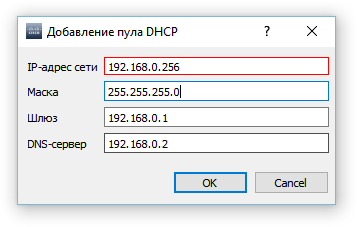
\includegraphics[width=0.8\linewidth]{pic/ipvalid}
\caption{Обозначение неправильного ввода}
\label{fig:ipvalid}
\end{figure}



\subsection{Генерация файла конфигурации}

Значения параметров маршрутизаторов, коммутаторов, интерфейсов, VLAN, DHCP, маршрутизации, NAT, ACL на протяжении работы программы хранятся в объектах класса \texttt{RouterModel}, \texttt{SwitchModel}, \texttt{InterfaceModel}, \texttt{VLANModel}, \texttt{DHCPModel}, \texttt{RouteModel}, \texttt{NATModel} и \texttt{ACLModel} соответственно, наследуемых от класса \texttt{ICiscoConfig}. Класс \texttt{ICiscoConfig} требует реализовать функцию \texttt{generetaeConfig}:

\begin{lstlisting}
virtual QString genereteConfig() = 0;
\end{lstlisting}

Вызов данной функции возвращает набор команд, необходимый для настройки соответствующего функционала.

Таким образом, после проверки правильности заполнения всех необходимых для ввода полей формы, производится запись в указанный пользователем файл значения функции \texttt{generateConfig()}.

%%\begin{lstlisting}
%%
%%!Writing Automated Startup
%%
%%enable
%%configure terminal
%%no ip domain-lookup
%%hostname hostname
%%enable secret class
%%end
%%\end{lstlisting}

%Исходя из схемы, представленной на рисунке \ref{fig:alghoritm}, выделяются 


\chapter{РУКОВОДСТВО ПОЛЬЗОВАТЕЛЯ}

После запуска программы появляется основное окно программы, в соответствии с рисунком \ref{fig:main}. 
%Пользователю доступны следующие действия:
%
%\begin{itemize}
%	\item добавление шаблона;
%	\item редактирование шаблона;
%	\item использование шаблона;
%	\item запуск справки;
%	\item показ информации о программе.
%\end{itemize}

\begin{figure}[ht!]
\centering
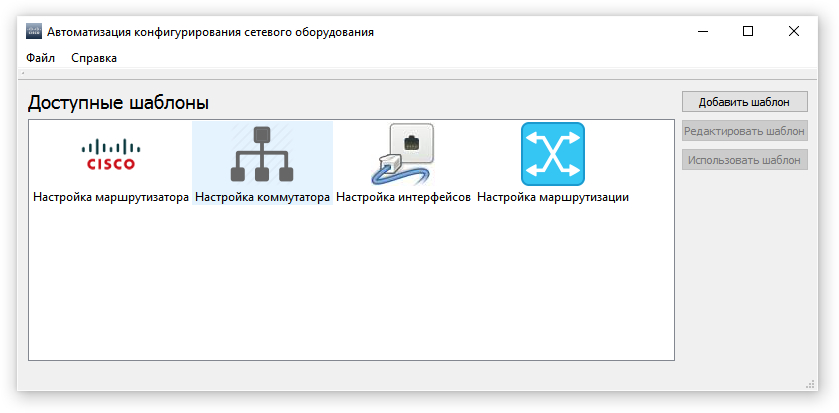
\includegraphics[width=0.8\linewidth]{pic/main}
\caption{Основное окно программы}
\label{fig:main}
\end{figure}

\section{Добавление шаблона}

\label{section:add_template}
\begin{enumerate}
	\item 
Для добавление нового шаблона нажмите кнопку \texttt{<<Добавить шаблон>>}, либо выберите пункт меню \texttt{Файл | Добавить новый шаблон}, либо нажмите сочетание клавиш \texttt{Crtl+N} (в соответствии с рисунком \ref{fig:add_template}).

\begin{figure}[h!]
	\centering
	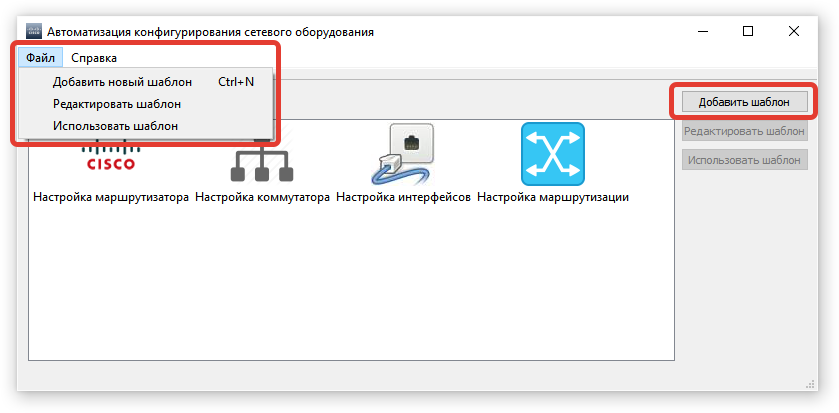
\includegraphics[width=0.8\linewidth]{pic/add_template}
	\caption{Добавление шаблона}
	\label{fig:add_template}
\end{figure}

	\item После этого появится окно добавления нового шаблона (в соответствии с рисунком \ref{fig:template_window}).

\begin{figure}[ht!]
\centering
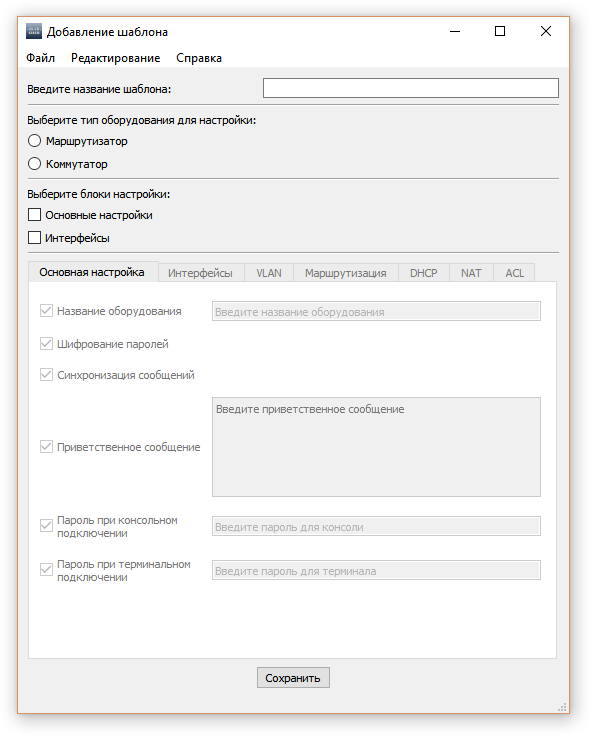
\includegraphics[width=1\linewidth]{pic/template_window}
\caption{Окно добавление шаблона}
\label{fig:template_window}
\end{figure}

	\item Введите название шаблона (в соответствии с рисунком \ref{fig:template_window_edit_name}) для дальнейшей его идентификации в списке других шаблонов.

\begin{figure}[ht!]
\centering
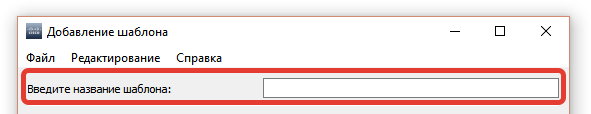
\includegraphics[width=1\linewidth]{pic/template_window_edit_name}
\caption{Ввод названия шаблона}
\label{fig:template_window_edit_name}
\end{figure}

	\item Выберите тип устройства для дальнейших действий (в соответствии с рисунком \ref{fig:template_window_edit_type}).

\begin{figure}[ht!]
\centering

\includegraphics[width=1\linewidth]{pic/template_window_edit_type}
\caption{Выбор типа устройства}
\label{fig:template_window_edit_type}
\end{figure}

Выбор типа <<Маршрутизатор>> позволяет выбирать следующие блоки настройки (в соответствии с рисунком \ref{fig:type_router}):
\begin{itemize}
	\item Основные настройки;
	\item Интерфейсы;
	\item Маршрутизация;
	\item DHCP;
	\item NAT;
	\item ACL.
\end{itemize}

\begin{figure}[th!]
\centering
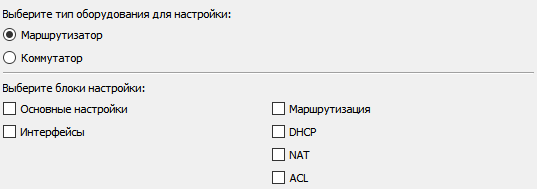
\includegraphics[width=1\linewidth]{pic/type_router}
\caption{Тип <<Маршрутизатор>>}
\label{fig:type_router}
\end{figure}

Выбор типа <<Коммутатор>> позволяет выбирать следующие блоки настройки (в соответствии с рисунком \ref{fig:type_switch}):
\begin{itemize}
	\item Основные настройки;
	\item Интерфейсы;
	\item VLAN.
\end{itemize}

\begin{figure}[th!]
\centering
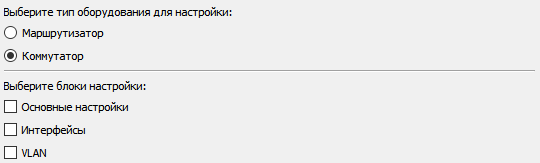
\includegraphics[width=1\linewidth]{pic/type_switch}
\caption{Тип <<Коммутатор>>}
\label{fig:type_switch}
\end{figure}

	\item Выберите блоки настройки из списка в зависимости от необходимого функционала (в соответствии с рисунками \ref{fig:type_router} и \ref{fig:type_switch})
\begin{enumerate}
	\item 	
	При выборе блока <<Основные настройки>> становится доступна доступна страница (в соответствии с рисунком \ref{fig:main_settings}), где можно настроить следующие для добавления в шаблон следующие параметры:
	
	\begin{itemize}
		\item название оборудования;
		\item шифрование паролей;
		\item синхронизация вывода сообщение при наборе команд;
		\item приветственное сообщение;
		\item пароль на консольное подключение;
		\item пароль на терминальное подключение.
	\end{itemize}
	
	По умолчанию, все параметры выбраны. Также можно настроить значения данных параметров по умолчанию.
	
\begin{figure}[th!]
\centering
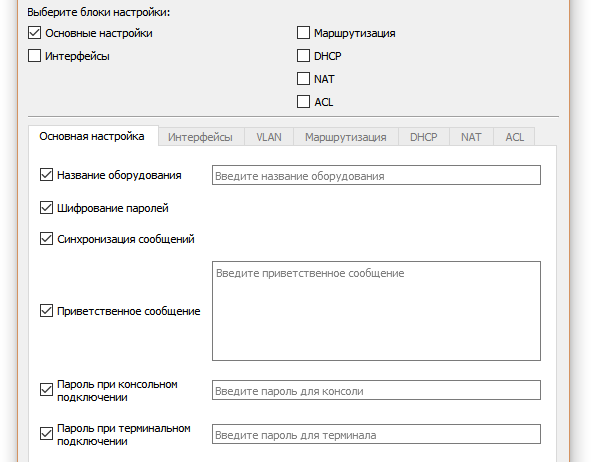
\includegraphics[width=1\linewidth]{pic/main_settings}
\caption{Основные настройки}
\label{fig:main_settings}
\end{figure}

\item 
При выборе блока <<Интерфейсы>> становится доступна страница (в соответствии с рисунком \ref{fig:interface_settings}), где можно добавлять или удалять интерфейсы, необходимые по данному шаблону.
%настроить следующие для добавления в шаблон следующие параметры:
%
%\begin{itemize}
%	\item название оборудования;
%	\item шифрование паролей;
%	\item синхронизация вывода сообщение при наборе команд;
%	\item приветственное сообщение;
%	\item пароль на консольное подключение;
%	\item пароль на терминальное подключение.
%\end{itemize}

\begin{figure}[th!]
\centering
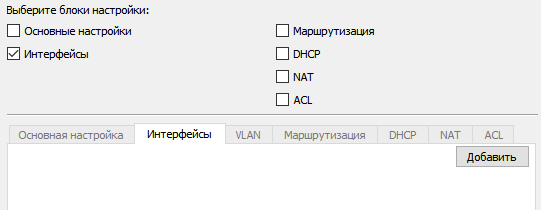
\includegraphics[width=1\linewidth]{pic/interface_settings}
\caption{Интерфейсы}
\label{fig:interface_settings}
\end{figure}

По умолчанию, интерфейсы отсутствуют. Для добавления необходимо нажать кнопку \texttt{<<Добавить>>} либо выбрать пункт меню \texttt{Редактирование | Добавить интерфейс}. 

При добавлении необходимо указать тип интерфейса и его номер. Опционально можно указать описание, режим и скорость передачи данных, IPv4-адрес с маской, IPv6-адрес, а также режим передачи трафика (тегированный или нет) c указанием соответствующих VLAN (в соответствии с рисунком \ref{fig:add_interface}).

\begin{figure}[th!]
	\centering
	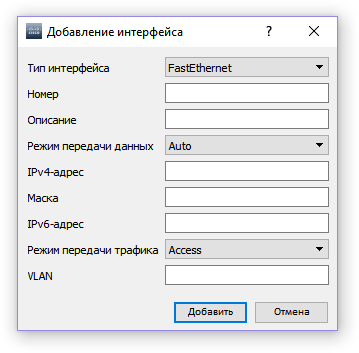
\includegraphics[width=0.8\linewidth]{pic/add_interface}
	\caption{Добавление интерфейса}
	\label{fig:add_interface}
\end{figure}

После нажатия в диалоге кнопки <<Добавить>> в списке интерфейсов появится добавленный интерфейс (в соответствии с рисунком \ref{fig:add_interface_2}).

Для дальнейшего редактирования интерфейса можно дважды кликнуть по названию интерфейса и откроется диалоговое окно, аналогичное окну при добавлении интерфейса. Также присутствует возможность удалить данный интерфейс из шаблона.

%Также можно настроить значения данных параметров по умолчанию.

\begin{figure}[th!]
\centering
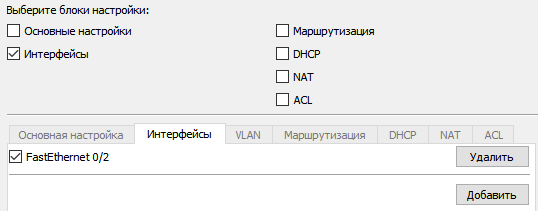
\includegraphics[width=1\linewidth]{pic/add_interface_2}
\caption{Список интерфейсов}
\label{fig:add_interface_2}
\end{figure}

\item 
При выборе блока <<VLAN>> становится доступна страница (в соответствии с рисунком \ref{fig:vlan_settings}), где можно добавлять или удалять VLAN'ы, необходимые по данному шаблону.

\begin{figure}[th!]
	\centering
	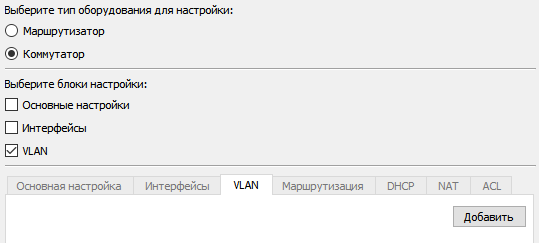
\includegraphics[width=1\linewidth]{pic/vlan_settings}
	\caption{VLAN}
	\label{fig:vlan_settings}
\end{figure}

По умолчанию, интерфейсы отсутствуют. Для добавления необходимо нажать кнопку \texttt{<<Добавить>>} либо выбрать пункт меню \texttt{Редактирование | Добавить VLAN}. 

При добавлении необходимо указать номер VLAN. Опционально можно указать название и описание VLAN. 

\begin{figure}[th!]
	\centering
	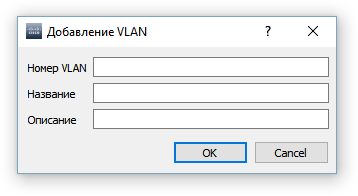
\includegraphics[width=0.8\linewidth]{pic/add_vlan}
	\caption{Добавление VLAN}
	\label{fig:add_vlan}
\end{figure}

После нажатия в диалоге кнопки <<Добавить>> в списке VLAN появится добавленный интерфейс (в соответствии с рисунком \ref{fig:add_vlan_2}).

Для дальнейшего редактирования VLAN можно дважды кликнуть по названию и откроется диалоговое окно, аналогичное окну при добавлении VLAN. Также присутствует возможность удалить данный VLAN из шаблона.

%Также можно настроить значения данных параметров по умолчанию.

\begin{figure}[th!]
	\centering
	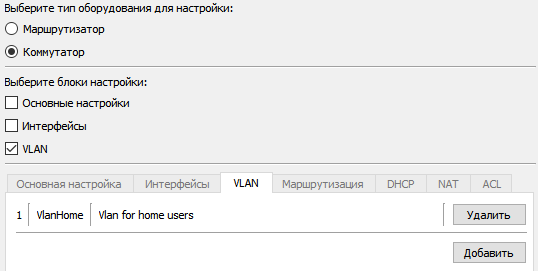
\includegraphics[width=1\linewidth]{pic/add_vlan_2}
	\caption{Список VLAN}
	\label{fig:add_vlan_2}
\end{figure}

\item 
При выборе блока <<Маршрутизация>> становится доступна страница (в соответствии с рисунком \ref{fig:route_settings}), где можно статическую и/или динамическую маршрутизацию.

\begin{figure}[th!]
	\centering
	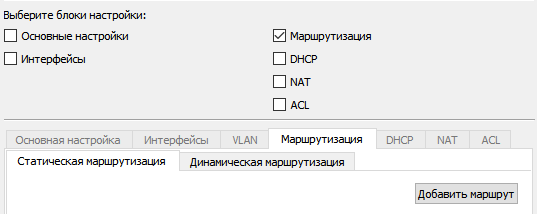
\includegraphics[width=1\linewidth]{pic/route_settings}
	\caption{Маршрутизация}
	\label{fig:route_settings}
\end{figure}

По умолчанию, статические маршруты отсутствуют. Для добавления необходимо нажать кнопку \texttt{<<Добавить>>} во вкладке \texttt{Статическая маршрутизация} либо выбрать пункт меню \texttt{Редактирование | Добавить статический маршрут}. 

При добавлении необходимо указать IP-адрес и маску сети назначения, а также выбрать, через что отправлять пакеты в данную сеть. Можно выбрать либо адрес следующего маршрутизатора с указанием соответствующего IP-адрес, либо интерфейс с указанием соответствующего интерфейса.

\begin{figure}[th!]
	\centering
	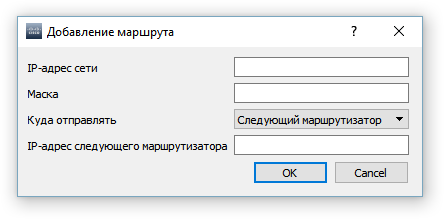
\includegraphics[width=\linewidth]{pic/add_route}
	\caption{Добавление статического маршрута}
	\label{fig:add_route}
\end{figure}

После нажатия в диалоге кнопки <<Добавить>> в списке маршрутов появится добавленный маршрут (в соответствии с рисунком \ref{fig:add_route_2}).

Для дальнейшего редактирования статического маршрута можно дважды кликнуть по названию и откроется диалоговое окно, аналогичное окну при добавлении статического маршрута. Также присутствует возможность удалить данный маршрут из шаблона.

%Также можно настроить значения данных параметров по умолчанию.

\begin{figure}[th!]
	\centering
	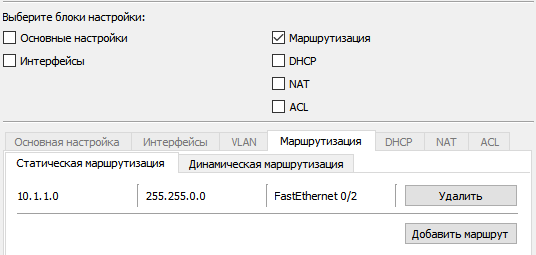
\includegraphics[width=1\linewidth]{pic/add_route_2}
	\caption{Список статических маршрутов}
	\label{fig:add_route_2}
\end{figure}

Для включения команд динамической маршрутизации в шаблон установите пункты OSPF или EIGRP (в соответствии с рисунком \ref{fig:dymanic_route}).

\begin{figure}[th!]
\centering
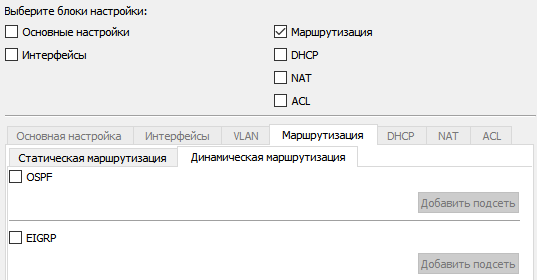
\includegraphics[width=1\linewidth]{pic/dymanic_route}
\caption{Динамическая маршрутизация}
\label{fig:dymanic_route}
\end{figure}

Для добавление сетей в объявления OSPF или EIGRP воспользуйтесь соответствующей кнопкой <<Добавить сеть>> или пунктом меню \texttt{Редактирование | Добавить сеть OSPF} (\texttt{Редактирование | Добавить сеть EIGRP}).

\item 
При выборе блока <<DCHP>> становится доступна страница (в соответствии с рисунком \ref{fig:dhcp_settings}), где можно настроить DHCP.

\begin{figure}[th!]
	\centering
	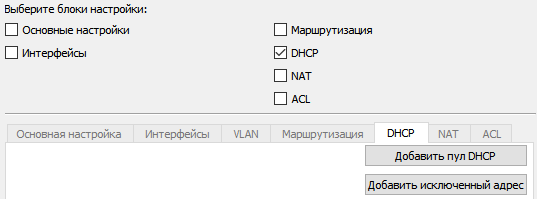
\includegraphics[width=1\linewidth]{pic/dhcp_settings}
	\caption{DHCP}
	\label{fig:dhcp_settings}
\end{figure}

По умолчанию, пулы DHCP отсутствуют. Для добавления пула DHCP, нажмите кнопку \texttt{<<Добавить пул DHCP>>} или выберите пункт меню \texttt{Редактирование | Добавить пул DHCP}. При добавлении необходимо указать IP-адрес сети с маской, а также IP-адрес шлюза. Опционально, можно указать DNS-сервер. После добавления IP-адрес шлюза будет автоматически включен в число исключенных адресов.

 Для добавления исключенного IP-адреса, нажмите кнопку \texttt{<<Добавить исключенный адрес>>} или выберите пункт меню \texttt{Редактирование | Добавить исключенный IP-адрес}.

\item 
При выборе блока <<NAT>> становится доступна страница (в соответствии с рисунком \ref{fig:nat_settings}), где можно настроить трансляцию сетевых адресов.

\begin{figure}[th!]
	\centering
	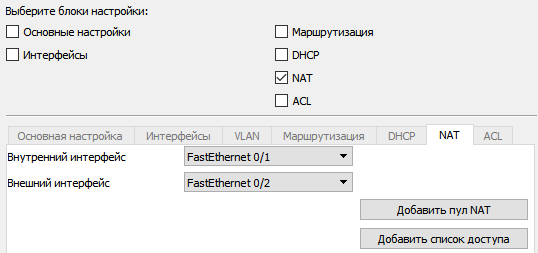
\includegraphics[width=1\linewidth]{pic/nat_settings}
	\caption{NAT}
	\label{fig:nat_settings}
\end{figure}

Укажите внешний и внутренний интерфейс, выбрав нужный из списка доступных.

Для добавления пула NAT, нажмите кнопку \texttt{<<Добавить пул NAT>>} или выберите пункт меню \texttt{Редактирование | Добавить пул NAT}.

Для добавления списка доступа нажмите кнопку \texttt{<<Добавить список доступа>>} или выберите пункт меню \texttt{Редактирование | Добавить список доступа}.

\item 
При выборе блока <<ACL>> становится доступна страница (в соответствии с рисунком \ref{fig:acl_settings}), где можно настроить ACL.

\begin{figure}[th!]
	\centering
	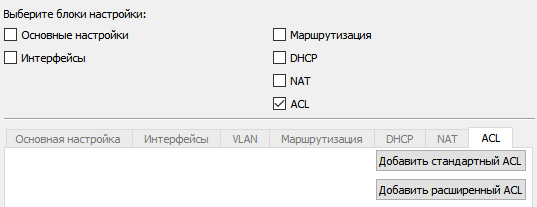
\includegraphics[width=1\linewidth]{pic/acl_settings}
	\caption{ACL}
	\label{fig:acl_settings}
\end{figure}

По умолчанию, ACL отсутствуют. Для добавления ACL, нажмите кнопку \texttt{<<Добавить стандарный ACL>>} или выберите пункт меню \texttt{Редактирование | Добавить стандартный ACL}. 

Для добавления расширенного ACL, нажмите кнопку \texttt{<<Добавить расширенного ACL>>} или выберите пункт меню \texttt{Редактирование | Добавить расширенный ACL}. 
\end{enumerate}

\item Нажмите кнопку <<Сохранить>> для сохранения изменений.

\end{enumerate}

\section{Редактирование шаблона}

Для редактирования шаблона:
\begin{enumerate}
	\item Выберите шаблон (в соответствии с рисунком \ref{fig:edit_template}).
	
	
\begin{figure}[th!]
\centering
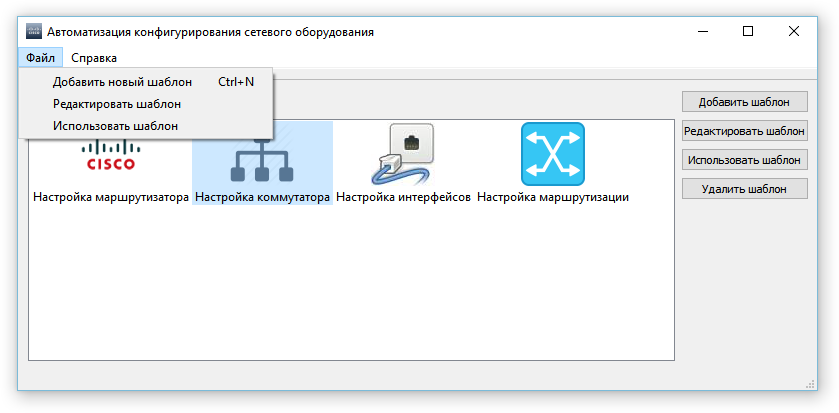
\includegraphics[width=1\linewidth]{pic/edit_template}
\caption{Выделение шаблона}
\label{fig:edit_template}
\end{figure}

	\item Нажмите кнопку \texttt{<<Редактировать шаблон>>} или выберите пункт меню \texttt{Файл | Редактировать шаблон}.
\end{enumerate}
Редактирование осуществляет в окне, аналогичном пункту <<Создание шаблона>> (смотри пункт \ref{section:add_template}).

\section{Использование шаблона}

Для использования шаблона:
\begin{enumerate}
	\item Выберите шаблон (в соответствии с рисунком \ref{fig:edit_template}).
	
	\item Нажмите кнопку \texttt{<<Использовать шаблон>>} или выберите пункт меню \texttt{Файл | Использовать шаблон}.
	
	\item В появившемся окне (пример приведен на рисунке \ref{fig:example}) введите или исправьте установленные по умолчанию значения на необходимые вам.
	
	
\begin{figure}[th!]
\centering
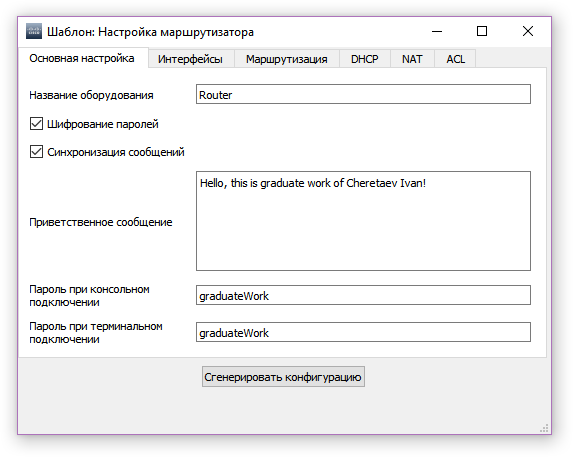
\includegraphics[width=1\linewidth]{pic/example}
\caption{Использование шаблона}
\label{fig:example}
\end{figure}
	
	\item Нажмите кнопку <<Сгенерировать конфигурацию>>.
	
	\item Выберите место сохранения файла и его имя.
\end{enumerate} 

\section{Удаление шаблона}

Для удаления шаблона:
\begin{enumerate}
	\item Выберите шаблон (в соответствии с рисунком \ref{fig:edit_template}).
	
	\item Нажмите кнопку \texttt{<<Удалить шаблон>>} или выберите пункт меню \texttt{Файл | Удалить шаблон}.
	
	\item Подтвердите удаление в появившемся диалоговом окне.
\end{enumerate} 

\section{Справка}

Для запуска справочной системы выберите пункт меню \texttt{Справка | Запуск справки} либо нажмите сочетание клавиш \texttt{Ctrl+H}. Отобразится начальное страница справки, представленная на рисунке \ref{fig:help}.

\begin{figure}[th!]
\centering
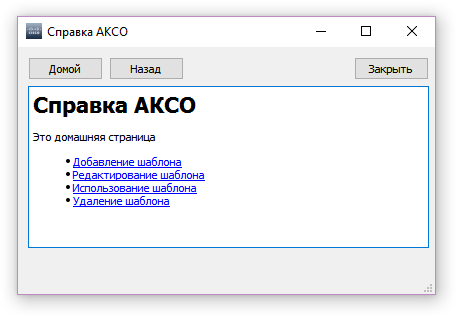
\includegraphics[width=0.8\linewidth]{pic/help}
\caption{Начальная страница справки}
\label{fig:help}
\end{figure}


Для просмотра краткой информации о программе выберите пункт меню \texttt{Справка | О программе}. Результат приведен на рисунке \ref{fig:about}.
\begin{figure}[th!]
\centering

\includegraphics[width=0.8\linewidth]{pic/about}
\caption{Окно <<О программе>>}
\label{fig:about}
\end{figure}


%\chapter{Конструкторский раздел}
\label{cha:design}

В данном разделе проектируется новая всячина.

\section{Архитектура всячины}

\paragraph{Проверка} параграфа. Вроде работает.
\paragraph{Вторая проверка} параграфа. Опять работает.

Вот.

\begin{itemize}
\item Это список с <<палочками>>.
\item Хотя он и не по ГОСТ, кажется.
\end{itemize}

\begin{enumerate}
\item Поэтому для списка, начинающегося с заглавной буквы, лучше список с цифрами.
\end{enumerate}

Формула \ref{F:F1} совершено бессмысленна.

%Кстати, при каких-то условиях <<удавалось>> получить двойный скобки вокруг номеров формул. Вопрос исследуется.

\begin{equation}
a= cb
\label{F:F1}
\end{equation}


Окружение \texttt{cases} опять работает (см. \ref{F:F2}), спасибо И. Короткову за исправления..


\begin{equation}
a= \begin{cases}
 3x + 5y + z, \mbox{если хорошо} \\
 7x - 2y + 4z, \mbox{если плохо}\\
 -6x + 3y + 2z, \mbox{если совсем плохо}
\end{cases}
\label{F:F2}
\end{equation}

\section{Подсистема всякой ерунды}

Культурная вставка dot-файлов через утилиту dot2tex (рис.~\ref{fig:fig02}).

\begin{figure}
  \centering
% [width=0.5\textwidth] --- регулировка ширины картинки
%  \includegraphics{inc/dot/cow2}
  \caption{Рисунок}
  \label{fig:fig02}
\end{figure}


\subsection{Блок-схема всякой ерунды}

\subsubsection*{Кстати о заголовках}

У нас есть и \Code{subsubsection}. Только лучше её не нумеровать.

%%% Local Variables:
%%% mode: latex
%%% TeX-master: "rpz"
%%% End:

%\chapter{Технологический раздел}
\label{cha:impl}

В данном разделе описано изготовление и требование всячины. Кстати,
в Latex нужно эскейпить подчёркивание (писать <<\verb|some\_function|>> для \Code{some\_function}).

\ifPDFTeX
Для вставки кода есть пакет \Code{listings}. К сожалению, пакет \Code{listings} всё ещё
работает криво при появлении в листинге русских букв и кодировке исходников utf-8.
В данном примере он (увы) на лету конвертируется в koi-8 в ходе сборки pdf.

Есть альтернатива \Code{listingsutf8}, однако она работает лишь с
\Code{\textbackslash{}lstinputlisting}, но не с окружением \Code{\textbackslash{}lstlisting}

Вот так можно вставлять псевдокод (питоноподобный язык определен в \Code{listings.inc.tex}):

\begin{lstlisting}[style=pseudocode,caption={Алгоритм оценки дипломных работ}]
def EvaluateDiplomas():
    for each student in Masters:
        student.Mark := 5
    for each student in Engineers:
        if Good(student):
            student.Mark := 5
        else:
            student.Mark := 4
\end{lstlisting}

Еще в шаблоне определен псевдоязык для BNF:

\begin{lstlisting}[style=grammar,basicstyle=\small,caption={Грамматика}]
  ifstmt -> "if" "(" expression ")" stmt |
            "if" "(" expression ")" stmt1 "else" stmt2
  number -> digit digit*
\end{lstlisting}

В листинге~\ref{lst:sample01} работают русские буквы. Сильная магия. Однако, работает
только во включаемых файлах, прямо в \TeX{} нельзя.

% Обратите внимание, что включается не ../src/..., а inc/src/...
% В Makefile есть соответствующее правило для inc/src/*,
% которое копирует исходные файлы из ../src и конвертирует из UTF-8 в KOI8-R.
% Кстати, поэтому использовать можно только русские буквы и ASCII,
% весь остальной UTF-8 вроде CJK и египетских иероглифов -- нельзя.

\lstinputlisting[language=C,caption=Пример (\Code{test.c}),label=lst:sample01]{customvalidator.cpp}

\else

Для вставки кода есть пакет \texttt{minted}. Он хорош всем кроме: необходимости Python (есть во всех нормальных (нет, Windows, я не про тебя) ОС) и Pygments и того, что нормально работает лишь в \XeLaTeX.

Можно пользоваться расширенным BFN:

\begin{listing}[H]
\begin{ebnfcode}
 letter = "A" | "B" | "C" | "D" | "E" | "F" | "G"
       | "H" | "I" | "J" | "K" | "L" | "M" | "N"
       | "O" | "P" | "Q" | "R" | "S" | "T" | "U"
       | "V" | "W" | "X" | "Y" | "Z" ;
digit = "0" | "1" | "2" | "3" | "4" | "5" | "6" | "7" | "8" | "9" ;
symbol = "[" | "]" | "{" | "}" | "(" | ")" | "<" | ">"
       | "'" | '"' | "=" | "|" | "." | "," | ";" ;
character = letter | digit | symbol | "_" ;
 
identifier = letter , { letter | digit | "_" } ;
terminal = "'" , character , { character } , "'" 
         | '"' , character , { character } , '"' ;
 
lhs = identifier ;
rhs = identifier
     | terminal
     | "[" , rhs , "]"
     | "{" , rhs , "}"
     | "(" , rhs , ")"
     | rhs , "|" , rhs
     | rhs , "," , rhs ;
 
rule = lhs , "=" , rhs , ";" ;
grammar = { rule } ;
\end{ebnfcode}
\caption{EBNF определённый через EBNF}
\label{lst:ebnf}
\end{listing}

А вот в листинге \ref{lst:c} на языке C работают русские комменты. Спасибо Pygments и Minted за это.

\begin{listing}[H]
\cfile{inc/src/test.c}
\caption{Пример — test.c} 
\end{listing}
\label{lst:c}

\fi

% Для вставки реального кода лучше использовать \texttt{\textbackslash lstinputlisting} (который понимает
% UTF8) и стили \Code{realcode} либо \Code{simplecode} (в зависимости от размера куска).




Можно также использовать окружение \Code{verbatim}, если \Code{listings} чем-то не
устраивает. Только следует помнить, что табы в нём <<съедаются>>. Существует так же команда \Code{\textbackslash{}verbatiminput} для вставки файла.

\begin{verbatim}
a_b = a + b; // русский комментарий
if (a_b > 0)
    a_b = 0;
\end{verbatim}

%%% Local Variables:
%%% mode: latex
%%% TeX-master: "rpz"
%%% End:

%\chapter{Экспериментальный раздел}
\label{cha:research}

В данном разделе проводятся вычислительные эксперименты.
А на рис.~\ref{fig:spire01} показана схема мыслительного процесса автора...

\begin{figure}
  \centering
%  \includegraphics[width=\textwidth]{inc/svg/pic01}
  \caption{Как страшно жить}
  \label{fig:spire01}
\end{figure}


%%% Local Variables:
%%% mode: latex
%%% TeX-master: "rpz"
%%% End:

%\chapter{Организационно-экономический раздел}
\label{cha:econom}

%%% Local Variables:
%%% mode: latex
%%% TeX-master: "rpz"
%%% End:

%\chapter{Промышленная экология и безопасность}\label{cha:bzd}


%%% Local Variables:
%%% mode: latex
%%% TeX-master: "rpz"
%%% End:


\backmatter %% Здесь заканчивается нумерованная часть документа и начинаются ссылки и
            %% заключение

\Conclusion % заключение к отчёту


В результате работы над выпускной квалификационной работой решена задача создания прикладного программного продукта для реализации пользовательского интерфейса, предоставляющего возможность создания, редактирования, использования и удаления шаблонов конфигурации оборудования, тем самым решая задачу автоматизации настройки сетевого оборудования Cisco.

%В результате проделанной работы по написанию выпускной квалификационной работы была создана программа~АКСО для создания конфигурационных файлов для сетевого оборудования Cisco на основании различных шаблонов и введенных пользователем данных.

Программа разработана в среде Qt Creator, что позволило создать кроссплатформенное приложение, на основе одного и того же исходного кода. Разработанное приложение на базе технологии объектно-ориентированного программирования обеспечивает удобный пользовательский интерфейс, реализующий заданный функционал:

\begin{itemize}
	\item создание шаблонов;
	\item редактирование и удаление шаблонов;
	\item контроль введенных значений, таких как текст, IP-адрес и т.д.;
	\item использование шаблонов для генерации файла, содержащего команды конфигурации.
\end{itemize}
%ввода данных: 
%%% Local Variables: 
%%% mode: latex
%%% TeX-master: "rpz"
%%% End: 


% % Список литературы при помощи BibTeX
% Юзать так:
%
% pdflatex rpz
% bibtex rpz
% pdflatex rpz

\bibliographystyle{gost780u}
\bibliography{rpz}

%%% Local Variables: 
%%% mode: latex
%%% TeX-master: "rpz"
%%% End: 


\appendix   % Тут идут приложения

%%--- Begin generated contents ---
%\chapter{Иерархический список классов}
%\section{Иерархия классов}
Иерархия классов.\begin{DoxyCompactList}
\item \contentsline{section}{Interface\+Model}{\pageref{class_interface_model}}{}
\item Q\+Abstract\+Table\+Model\begin{DoxyCompactList}
\item \contentsline{section}{Interface\+Model\+List}{\pageref{class_interface_model_list}}{}
\end{DoxyCompactList}
\item \contentsline{section}{Q\+List$<$ T $>$}{\pageref{class_q_list}}{}
\item \contentsline{section}{Q\+List$<$ Interface\+Model $\ast$ $>$}{\pageref{class_q_list}}{}
\item Q\+Main\+Window\begin{DoxyCompactList}
\item \contentsline{section}{Main\+Window}{\pageref{class_main_window}}{}
\end{DoxyCompactList}
\item Q\+Object\begin{DoxyCompactList}
\item \contentsline{section}{Network\+Equipment\+Model}{\pageref{class_network_equipment_model}}{}
\end{DoxyCompactList}
\item Q\+Validator\begin{DoxyCompactList}
\item \contentsline{section}{Ipv4\+Validator}{\pageref{class_ipv4_validator}}{}
\item \contentsline{section}{Ipv6\+Validator}{\pageref{class_ipv6_validator}}{}
\item \contentsline{section}{Text\+Validator}{\pageref{class_text_validator}}{}
\item \contentsline{section}{Word\+Validator}{\pageref{class_word_validator}}{}
\end{DoxyCompactList}
\item Q\+Widget\begin{DoxyCompactList}
\item \contentsline{section}{Network\+Equipment\+Form}{\pageref{class_network_equipment_form}}{}
\end{DoxyCompactList}
\end{DoxyCompactList}

%\chapter{Алфавитный указатель классов}
%\section{Классы}
Классы с их кратким описанием.\begin{DoxyCompactList}
\item\contentsline{section}{\hyperlink{class_interface_model}{Interface\+Model} }{\pageref{class_interface_model}}{}
\item\contentsline{section}{\hyperlink{class_interface_model_list}{Interface\+Model\+List} }{\pageref{class_interface_model_list}}{}
\item\contentsline{section}{\hyperlink{class_ipv4_validator}{Ipv4\+Validator} }{\pageref{class_ipv4_validator}}{}
\item\contentsline{section}{\hyperlink{class_ipv6_validator}{Ipv6\+Validator} }{\pageref{class_ipv6_validator}}{}
\item\contentsline{section}{\hyperlink{class_main_window}{Main\+Window} }{\pageref{class_main_window}}{}
\item\contentsline{section}{\hyperlink{class_network_equipment_form}{Network\+Equipment\+Form} }{\pageref{class_network_equipment_form}}{}
\item\contentsline{section}{\hyperlink{class_network_equipment_model}{Network\+Equipment\+Model} \\*Модель сетевого оборудования }{\pageref{class_network_equipment_model}}{}
\item\contentsline{section}{\hyperlink{class_q_list}{Q\+List$<$ T $>$} }{\pageref{class_q_list}}{}
\item\contentsline{section}{\hyperlink{class_text_validator}{Text\+Validator} }{\pageref{class_text_validator}}{}
\item\contentsline{section}{\hyperlink{class_word_validator}{Word\+Validator} }{\pageref{class_word_validator}}{}
\end{DoxyCompactList}

\chapter{Документация исходного кода}
\label{cha:documentation}
\hypertarget{class_interface_model}{}\section{Класс Interface\+Model}
\label{class_interface_model}\index{Interface\+Model@{Interface\+Model}}
\subsection*{Открытые члены}
\begin{DoxyCompactItemize}
\item 
Interface\+Type {\bfseries type} ()\hypertarget{class_interface_model_ab9a3cf858cda42f7f21d86c701ed9baa}{}\label{class_interface_model_ab9a3cf858cda42f7f21d86c701ed9baa}

\item 
void {\bfseries set\+Type} (Interface\+Type type)\hypertarget{class_interface_model_a6d1e3a33e22e61dfbc860a23016b936e}{}\label{class_interface_model_a6d1e3a33e22e61dfbc860a23016b936e}

\item 
Q\+String {\bfseries number} ()\hypertarget{class_interface_model_ab7d36b21ece7aaeff0ad1399eaee6877}{}\label{class_interface_model_ab7d36b21ece7aaeff0ad1399eaee6877}

\item 
void {\bfseries set\+Number} (Q\+String number)\hypertarget{class_interface_model_a7bf6cec7997845df02b48a09c8edbb6d}{}\label{class_interface_model_a7bf6cec7997845df02b48a09c8edbb6d}

\item 
Q\+String {\bfseries description} ()\hypertarget{class_interface_model_a3d75ae4692a1b497a5677dda6592ee32}{}\label{class_interface_model_a3d75ae4692a1b497a5677dda6592ee32}

\item 
void {\bfseries set\+Description} (Q\+String description)\hypertarget{class_interface_model_a720fa2dcb0864bc64204e248314ac5a7}{}\label{class_interface_model_a720fa2dcb0864bc64204e248314ac5a7}

\item 
Duplex {\bfseries duplex} ()\hypertarget{class_interface_model_ae3ccb29aa96cf1d859091d5ebc213fde}{}\label{class_interface_model_ae3ccb29aa96cf1d859091d5ebc213fde}

\item 
void {\bfseries set\+Duplex} (Duplex duplex)\hypertarget{class_interface_model_a9f82d7f6f71fe196a55ed6bbc32a2809}{}\label{class_interface_model_a9f82d7f6f71fe196a55ed6bbc32a2809}

\item 
Q\+Host\+Address {\bfseries ipv4} ()\hypertarget{class_interface_model_a1601e72efd97a651dbc4541387afe47b}{}\label{class_interface_model_a1601e72efd97a651dbc4541387afe47b}

\item 
void {\bfseries set\+Ipv4} (Q\+Host\+Address ip)\hypertarget{class_interface_model_a0e4826c6024f3ea4a229df52809f8c17}{}\label{class_interface_model_a0e4826c6024f3ea4a229df52809f8c17}

\item 
Q\+Host\+Address {\bfseries ipv6} ()\hypertarget{class_interface_model_a4c5651b1ced869c27937443f073dd609}{}\label{class_interface_model_a4c5651b1ced869c27937443f073dd609}

\item 
void {\bfseries set\+Ipv6} (Q\+Host\+Address ip)\hypertarget{class_interface_model_af486a90f09c150d2e45a780b73145bb0}{}\label{class_interface_model_af486a90f09c150d2e45a780b73145bb0}

\end{DoxyCompactItemize}


Объявления и описания членов классов находятся в файлах\+:\begin{DoxyCompactItemize}
\item 
interfacemodel.\+h\item 
interfacemodel.\+cpp\end{DoxyCompactItemize}

\hypertarget{class_interface_model_list}{}\section{Класс Interface\+Model\+List}
\label{class_interface_model_list}\index{Interface\+Model\+List@{Interface\+Model\+List}}
Граф наследования\+:Interface\+Model\+List\+:\begin{figure}[H]
\begin{center}
\leavevmode
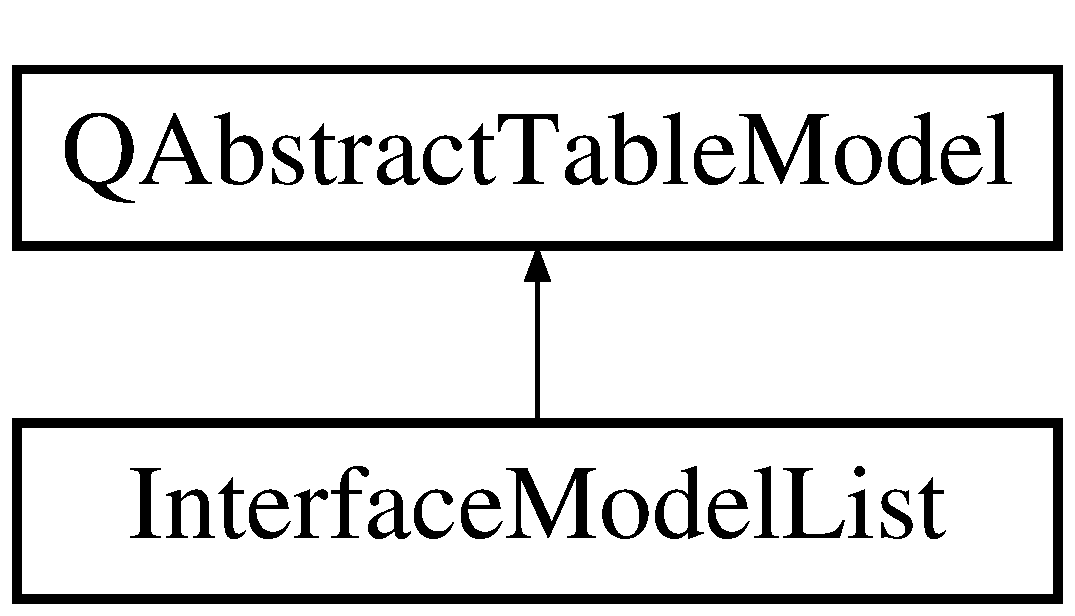
\includegraphics[height=2.000000cm]{class_interface_model_list}
\end{center}
\end{figure}
\subsection*{Открытые члены}
\begin{DoxyCompactItemize}
\item 
{\bfseries Interface\+Model\+List} (Q\+Object $\ast$parent)\hypertarget{class_interface_model_list_a926a7248c32335cb27669f0220b2a1b5}{}\label{class_interface_model_list_a926a7248c32335cb27669f0220b2a1b5}

\item 
int {\bfseries row\+Count} (const Q\+Model\+Index \&parent=Q\+Model\+Index()) const \hypertarget{class_interface_model_list_ad8846f668c2fbffdd8de7cb602e775d4}{}\label{class_interface_model_list_ad8846f668c2fbffdd8de7cb602e775d4}

\item 
int {\bfseries column\+Count} (const Q\+Model\+Index \&parent=Q\+Model\+Index()) const \hypertarget{class_interface_model_list_a590c92f0cca76b9838a1537bd5d34518}{}\label{class_interface_model_list_a590c92f0cca76b9838a1537bd5d34518}

\item 
Q\+Variant {\bfseries data} (const Q\+Model\+Index \&index, int role=Qt\+::\+Display\+Role) const \hypertarget{class_interface_model_list_a4c319165cc4c9ce42530ba40c5f6ae48}{}\label{class_interface_model_list_a4c319165cc4c9ce42530ba40c5f6ae48}

\item 
void {\bfseries set\+Interfaces} (\hyperlink{class_q_list}{Q\+List}$<$ \hyperlink{class_interface_model}{Interface\+Model} $\ast$ $>$ interfaces)\hypertarget{class_interface_model_list_a90c904fdb3e2c825d565e8acadab864e}{}\label{class_interface_model_list_a90c904fdb3e2c825d565e8acadab864e}

\end{DoxyCompactItemize}


Объявления и описания членов классов находятся в файлах\+:\begin{DoxyCompactItemize}
\item 
interfacemodel.\+h\item 
interfacemodel.\+cpp\end{DoxyCompactItemize}

\hypertarget{class_ipv4_validator}{}\section{Класс Ipv4\+Validator}
\label{class_ipv4_validator}\index{Ipv4\+Validator@{Ipv4\+Validator}}
Граф наследования\+:Ipv4\+Validator\+:\begin{figure}[H]
\begin{center}
\leavevmode
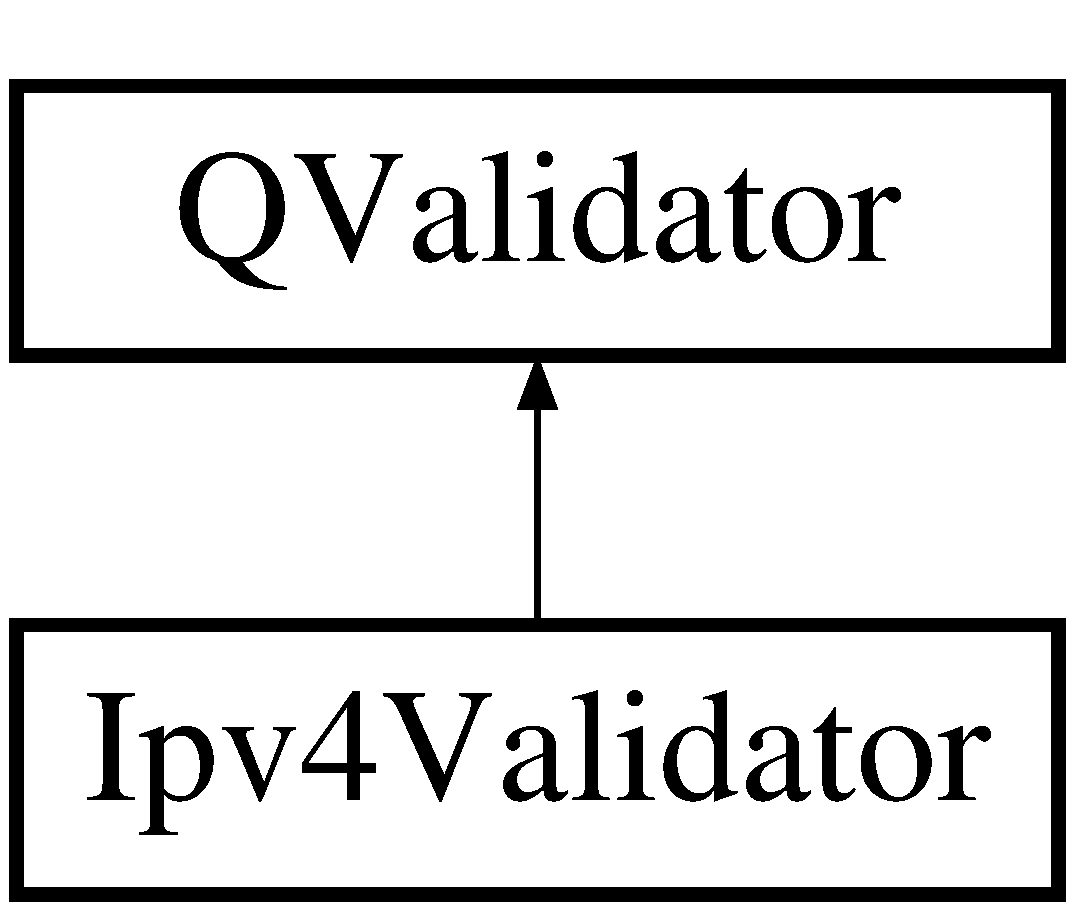
\includegraphics[height=2.000000cm]{class_ipv4_validator}
\end{center}
\end{figure}
\subsection*{Открытые члены}
\begin{DoxyCompactItemize}
\item 
\hyperlink{class_ipv4_validator_a5be0312dd5dfc0879eb9dc728a4ff577}{Ipv4\+Validator} (Q\+Object $\ast$parent=0)
\begin{DoxyCompactList}\small\item\em \hyperlink{class_ipv4_validator_a5be0312dd5dfc0879eb9dc728a4ff577}{Ipv4\+Validator\+::\+Ipv4\+Validator}. \end{DoxyCompactList}\item 
State \hyperlink{class_ipv4_validator_a6e5095efeaf75e97c1842b8c42db7c03}{validate} (Q\+String \&, int \&) const 
\begin{DoxyCompactList}\small\item\em \hyperlink{class_ipv4_validator_a6e5095efeaf75e97c1842b8c42db7c03}{Ipv4\+Validator\+::validate}. \end{DoxyCompactList}\end{DoxyCompactItemize}


\subsection{Конструктор(ы)}
\index{Ipv4\+Validator@{Ipv4\+Validator}!Ipv4\+Validator@{Ipv4\+Validator}}
\index{Ipv4\+Validator@{Ipv4\+Validator}!Ipv4\+Validator@{Ipv4\+Validator}}
\subsubsection[{\texorpdfstring{Ipv4\+Validator(\+Q\+Object $\ast$parent=0)}{Ipv4Validator(QObject *parent=0)}}]{\setlength{\rightskip}{0pt plus 5cm}Ipv4\+Validator\+::\+Ipv4\+Validator (
\begin{DoxyParamCaption}
\item[{Q\+Object $\ast$}]{parent = {\ttfamily 0}}
\end{DoxyParamCaption}
)}\hypertarget{class_ipv4_validator_a5be0312dd5dfc0879eb9dc728a4ff577}{}\label{class_ipv4_validator_a5be0312dd5dfc0879eb9dc728a4ff577}


\hyperlink{class_ipv4_validator_a5be0312dd5dfc0879eb9dc728a4ff577}{Ipv4\+Validator\+::\+Ipv4\+Validator}. 


\begin{DoxyParams}{Аргументы}
{\em parent} & \\
\hline
\end{DoxyParams}


\subsection{Методы}
\index{Ipv4\+Validator@{Ipv4\+Validator}!validate@{validate}}
\index{validate@{validate}!Ipv4\+Validator@{Ipv4\+Validator}}
\subsubsection[{\texorpdfstring{validate(\+Q\+String \&, int \&) const }{validate(QString &, int &) const }}]{\setlength{\rightskip}{0pt plus 5cm}Q\+Validator\+::\+State Ipv4\+Validator\+::validate (
\begin{DoxyParamCaption}
\item[{Q\+String \&}]{text, }
\item[{int \&}]{pos}
\end{DoxyParamCaption}
) const}\hypertarget{class_ipv4_validator_a6e5095efeaf75e97c1842b8c42db7c03}{}\label{class_ipv4_validator_a6e5095efeaf75e97c1842b8c42db7c03}


\hyperlink{class_ipv4_validator_a6e5095efeaf75e97c1842b8c42db7c03}{Ipv4\+Validator\+::validate}. 


\begin{DoxyParams}{Аргументы}
{\em text} & \\
\hline
{\em pos} & \\
\hline
\end{DoxyParams}
\begin{DoxyReturn}{Возвращает}

\end{DoxyReturn}


Объявления и описания членов классов находятся в файлах\+:\begin{DoxyCompactItemize}
\item 
customvalidator.\+h\item 
customvalidator.\+cpp\end{DoxyCompactItemize}

\hypertarget{class_ipv6_validator}{}\section{Класс Ipv6\+Validator}
\label{class_ipv6_validator}\index{Ipv6\+Validator@{Ipv6\+Validator}}
Граф наследования\+:Ipv6\+Validator\+:\begin{figure}[H]
\begin{center}
\leavevmode
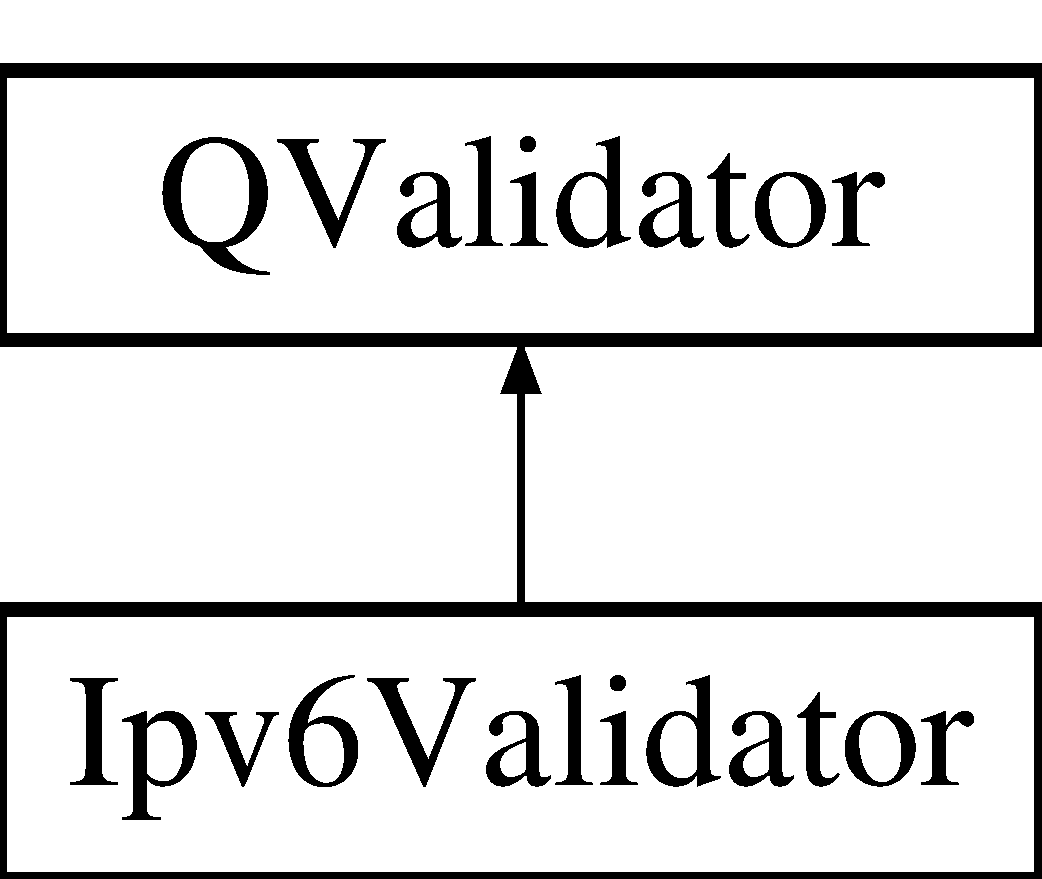
\includegraphics[height=2.000000cm]{class_ipv6_validator}
\end{center}
\end{figure}
\subsection*{Открытые члены}
\begin{DoxyCompactItemize}
\item 
\hyperlink{class_ipv6_validator_a2caeac54ee2995a6ac4b7716a52314f3}{Ipv6\+Validator} (Q\+Object $\ast$parent=0)
\begin{DoxyCompactList}\small\item\em \hyperlink{class_ipv6_validator_a2caeac54ee2995a6ac4b7716a52314f3}{Ipv6\+Validator\+::\+Ipv6\+Validator}. \end{DoxyCompactList}\item 
State \hyperlink{class_ipv6_validator_a847681eac42c4b238a3b3e8c8c5d18c2}{validate} (Q\+String \&, int \&) const 
\begin{DoxyCompactList}\small\item\em \hyperlink{class_ipv6_validator_a847681eac42c4b238a3b3e8c8c5d18c2}{Ipv6\+Validator\+::validate}. \end{DoxyCompactList}\end{DoxyCompactItemize}


\subsection{Конструктор(ы)}
\index{Ipv6\+Validator@{Ipv6\+Validator}!Ipv6\+Validator@{Ipv6\+Validator}}
\index{Ipv6\+Validator@{Ipv6\+Validator}!Ipv6\+Validator@{Ipv6\+Validator}}
\subsubsection[{\texorpdfstring{Ipv6\+Validator(\+Q\+Object $\ast$parent=0)}{Ipv6Validator(QObject *parent=0)}}]{\setlength{\rightskip}{0pt plus 5cm}Ipv6\+Validator\+::\+Ipv6\+Validator (
\begin{DoxyParamCaption}
\item[{Q\+Object $\ast$}]{parent = {\ttfamily 0}}
\end{DoxyParamCaption}
)}\hypertarget{class_ipv6_validator_a2caeac54ee2995a6ac4b7716a52314f3}{}\label{class_ipv6_validator_a2caeac54ee2995a6ac4b7716a52314f3}


\hyperlink{class_ipv6_validator_a2caeac54ee2995a6ac4b7716a52314f3}{Ipv6\+Validator\+::\+Ipv6\+Validator}. 


\begin{DoxyParams}{Аргументы}
{\em parent} & \\
\hline
\end{DoxyParams}


\subsection{Методы}
\index{Ipv6\+Validator@{Ipv6\+Validator}!validate@{validate}}
\index{validate@{validate}!Ipv6\+Validator@{Ipv6\+Validator}}
\subsubsection[{\texorpdfstring{validate(\+Q\+String \&, int \&) const }{validate(QString &, int &) const }}]{\setlength{\rightskip}{0pt plus 5cm}Q\+Validator\+::\+State Ipv6\+Validator\+::validate (
\begin{DoxyParamCaption}
\item[{Q\+String \&}]{text, }
\item[{int \&}]{pos}
\end{DoxyParamCaption}
) const}\hypertarget{class_ipv6_validator_a847681eac42c4b238a3b3e8c8c5d18c2}{}\label{class_ipv6_validator_a847681eac42c4b238a3b3e8c8c5d18c2}


\hyperlink{class_ipv6_validator_a847681eac42c4b238a3b3e8c8c5d18c2}{Ipv6\+Validator\+::validate}. 


\begin{DoxyParams}{Аргументы}
{\em text} & \\
\hline
{\em pos} & \\
\hline
\end{DoxyParams}
\begin{DoxyReturn}{Возвращает}

\end{DoxyReturn}


Объявления и описания членов классов находятся в файлах\+:\begin{DoxyCompactItemize}
\item 
customvalidator.\+h\item 
customvalidator.\+cpp\end{DoxyCompactItemize}

\hypertarget{class_main_window}{}\section{Класс Main\+Window}
\label{class_main_window}\index{Main\+Window@{Main\+Window}}
Граф наследования\+:Main\+Window\+:\begin{figure}[H]
\begin{center}
\leavevmode
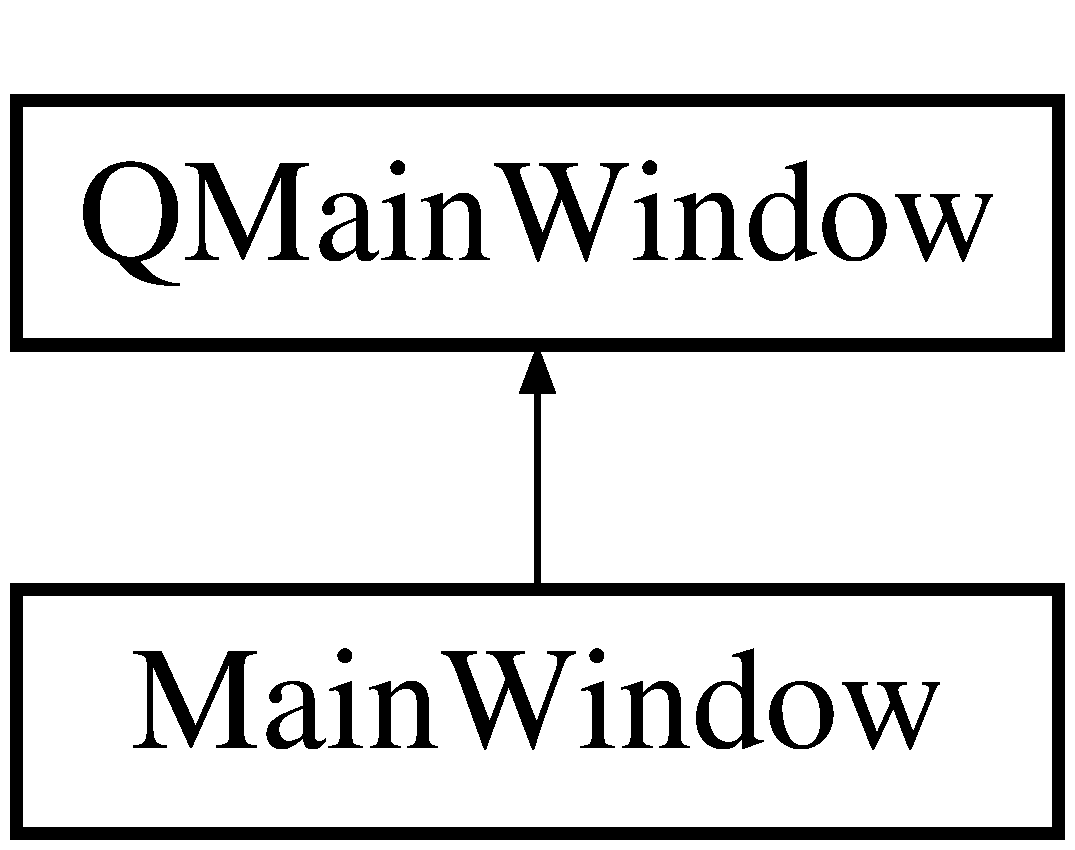
\includegraphics[height=2.000000cm]{class_main_window}
\end{center}
\end{figure}
\subsection*{Открытые члены}
\begin{DoxyCompactItemize}
\item 
{\bfseries Main\+Window} (Q\+Widget $\ast$parent=0)\hypertarget{class_main_window_a8b244be8b7b7db1b08de2a2acb9409db}{}\label{class_main_window_a8b244be8b7b7db1b08de2a2acb9409db}

\end{DoxyCompactItemize}


Объявления и описания членов классов находятся в файлах\+:\begin{DoxyCompactItemize}
\item 
mainwindow.\+h\item 
mainwindow.\+cpp\end{DoxyCompactItemize}

\hypertarget{class_network_equipment_form}{}\section{Класс Network\+Equipment\+Form}
\label{class_network_equipment_form}\index{Network\+Equipment\+Form@{Network\+Equipment\+Form}}
Граф наследования\+:Network\+Equipment\+Form\+:\begin{figure}[H]
\begin{center}
\leavevmode
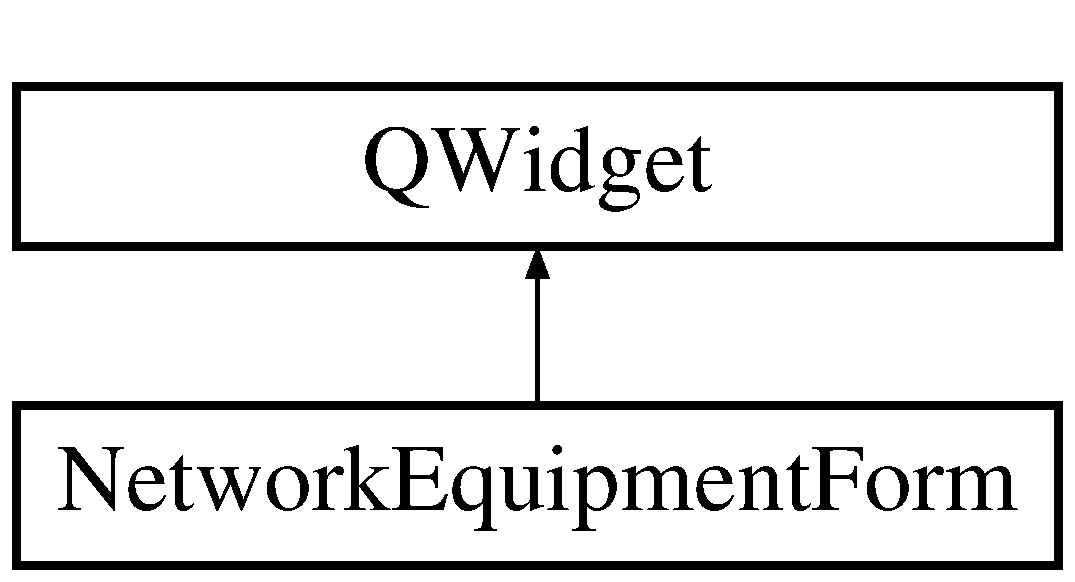
\includegraphics[height=2.000000cm]{class_network_equipment_form}
\end{center}
\end{figure}
\subsection*{Открытые слоты}
\begin{DoxyCompactItemize}
\item 
virtual void {\bfseries set\+Need\+Hostname} (bool need\+Hostname)\hypertarget{class_network_equipment_form_aa4f27acc75a23ad6217c73d1993d0376}{}\label{class_network_equipment_form_aa4f27acc75a23ad6217c73d1993d0376}

\item 
virtual void {\bfseries set\+Hostname} (Q\+String hostname)\hypertarget{class_network_equipment_form_a1752541512a46670f6febf6b72cf5982}{}\label{class_network_equipment_form_a1752541512a46670f6febf6b72cf5982}

\item 
virtual void {\bfseries set\+Password\+Encryption} (bool password\+Encryption)\hypertarget{class_network_equipment_form_a0d9eb5989eb412d6280932312e9b20ac}{}\label{class_network_equipment_form_a0d9eb5989eb412d6280932312e9b20ac}

\item 
virtual void {\bfseries set\+Need\+Banner\+Motd} (bool need\+Banner\+Motd)\hypertarget{class_network_equipment_form_a2afda0d1433c5d628a64fdd8257c3eea}{}\label{class_network_equipment_form_a2afda0d1433c5d628a64fdd8257c3eea}

\item 
virtual void {\bfseries set\+Banner\+Motd} (Q\+String banner\+Motd)\hypertarget{class_network_equipment_form_a79f90ee6080427b546440919fda03a63}{}\label{class_network_equipment_form_a79f90ee6080427b546440919fda03a63}

\item 
virtual void {\bfseries set\+Logging\+Synchronous} (bool logging\+Synchronous)\hypertarget{class_network_equipment_form_a648fbcdd8f69b64eab22da3ebb1f962f}{}\label{class_network_equipment_form_a648fbcdd8f69b64eab22da3ebb1f962f}

\item 
virtual void {\bfseries set\+Need\+Password\+Console} (bool need\+Password\+Console)\hypertarget{class_network_equipment_form_a47fbe2df13e3571ee14f74b40e0ee85c}{}\label{class_network_equipment_form_a47fbe2df13e3571ee14f74b40e0ee85c}

\item 
virtual void {\bfseries set\+Password\+Console} (Q\+String password)\hypertarget{class_network_equipment_form_a433f72d8df210acf7a77fcb96da9cd1b}{}\label{class_network_equipment_form_a433f72d8df210acf7a77fcb96da9cd1b}

\item 
virtual void {\bfseries set\+Need\+Password\+Vty} (bool need\+Password\+Vty)\hypertarget{class_network_equipment_form_a4c0fe8aa82ac42bd34f8f44f3f42e966}{}\label{class_network_equipment_form_a4c0fe8aa82ac42bd34f8f44f3f42e966}

\item 
virtual void {\bfseries set\+Password\+Vty} (Q\+String password)\hypertarget{class_network_equipment_form_a4a33264c3f13fc8795d3fce4d4a451cf}{}\label{class_network_equipment_form_a4a33264c3f13fc8795d3fce4d4a451cf}

\end{DoxyCompactItemize}
\subsection*{Открытые члены}
\begin{DoxyCompactItemize}
\item 
{\bfseries Network\+Equipment\+Form} (Q\+Widget $\ast$parent=0)\hypertarget{class_network_equipment_form_a1ee2a5fc8df7255d2887ff9a898c1139}{}\label{class_network_equipment_form_a1ee2a5fc8df7255d2887ff9a898c1139}

\item 
void {\bfseries set\+Model} (\hyperlink{class_network_equipment_model}{Network\+Equipment\+Model} $\ast$model)\hypertarget{class_network_equipment_form_a36fc9eb8d7f2a5ff79084661709a9936}{}\label{class_network_equipment_form_a36fc9eb8d7f2a5ff79084661709a9936}

\end{DoxyCompactItemize}


\subsection{Подробное описание}
Представление (View) в триаде M\+VP сетевого оборудования 

Объявления и описания членов классов находятся в файлах\+:\begin{DoxyCompactItemize}
\item 
networkequipmentform.\+h\item 
networkequipmentform.\+cpp\end{DoxyCompactItemize}

\hypertarget{class_network_equipment_model}{}\section{Класс Network\+Equipment\+Model}
\label{class_network_equipment_model}\index{Network\+Equipment\+Model@{Network\+Equipment\+Model}}


Модель сетевого оборудования  


Граф наследования\+:Network\+Equipment\+Model\+:\begin{figure}[H]
\begin{center}
\leavevmode
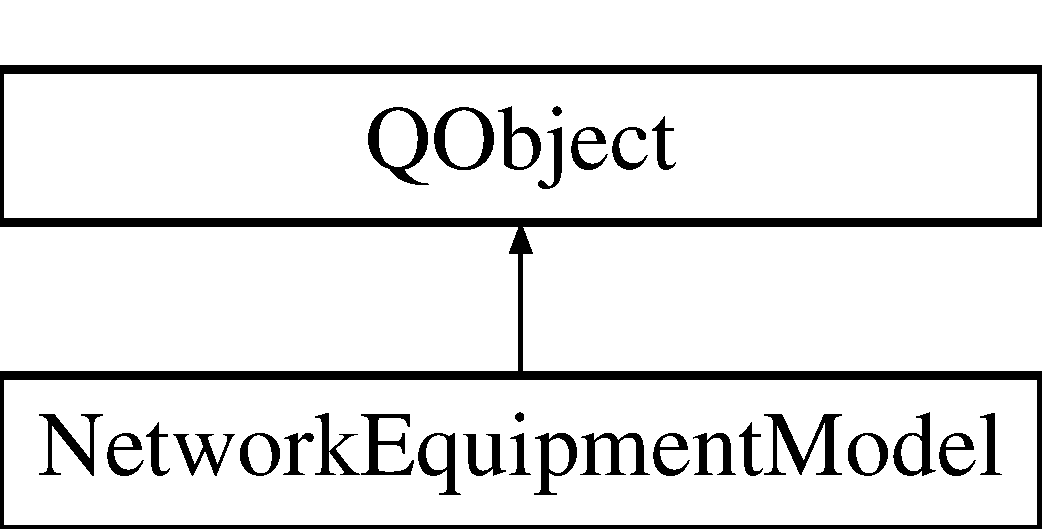
\includegraphics[height=2.000000cm]{class_network_equipment_model}
\end{center}
\end{figure}
\subsection*{Открытые слоты}
\begin{DoxyCompactItemize}
\item 
virtual void \hyperlink{class_network_equipment_model_a952a89f03887ab83ed42d404aad7acf4}{set\+Need\+Hostname} (bool \hyperlink{class_network_equipment_model_a67cb5cf3284a19a1a0d6a7b22fa2a91e}{need\+Hostname})
\begin{DoxyCompactList}\small\item\em Оболочка для установления необходимости называть оборудование \end{DoxyCompactList}\item 
virtual void \hyperlink{class_network_equipment_model_a844d05c49e462ea50dbf07b73597f65c}{set\+Hostname} (Q\+String \hyperlink{class_network_equipment_model_a59f5581ce5f16229235bc9ace24e11d6}{hostname})
\begin{DoxyCompactList}\small\item\em Оболочка для установки нового названия оборудования \end{DoxyCompactList}\item 
virtual void \hyperlink{class_network_equipment_model_a0303cb675bc0d42bff6b90d6e7b8bbb1}{set\+Password\+Encryption} (bool \hyperlink{class_network_equipment_model_a46900023e99e2791d5e0ff85204f25fb}{password\+Encryption})
\begin{DoxyCompactList}\small\item\em Оболочка для изменения необходимости скрывать пароли \end{DoxyCompactList}\item 
virtual void \hyperlink{class_network_equipment_model_a45955890b14b8dbd4f76df92cff2a82e}{set\+Need\+Banner\+Motd} (bool \hyperlink{class_network_equipment_model_ab20b1087ae50a8546bdabfa598e8c647}{need\+Banner\+Motd})
\begin{DoxyCompactList}\small\item\em Оболочка для установление необходимости указывать приветственное сообщение \end{DoxyCompactList}\item 
virtual void \hyperlink{class_network_equipment_model_a73bfb9a80a611f8925e23b4e68c95821}{set\+Banner\+Motd} (Q\+String \hyperlink{class_network_equipment_model_a9256503fdb609788939777565574ae7c}{banner\+Motd})
\begin{DoxyCompactList}\small\item\em Оболочка для изменения текущего текста приветствия \end{DoxyCompactList}\item 
virtual void \hyperlink{class_network_equipment_model_abe5f1892f0ca1bf727b8ceaf7baac189}{set\+Logging\+Synchronous} (bool \hyperlink{class_network_equipment_model_a7321ba74141fd1bc694a6607363625ae}{logging\+Synchronous})
\begin{DoxyCompactList}\small\item\em Оболочка для изменения запрета вывода каких-\/либо консольных сообщений при вводе команд в консольном режиме \end{DoxyCompactList}\item 
virtual void \hyperlink{class_network_equipment_model_afcdfd40284207e699e956dd3877a96c2}{set\+Need\+Password\+Console} (bool \hyperlink{class_network_equipment_model_ada70138a6ca4a8ad1bd07fa48998c9d8}{need\+Password\+Console})
\begin{DoxyCompactList}\small\item\em Оболочка для изменения необходимости ввода пароля при консольном подключении \end{DoxyCompactList}\item 
virtual void \hyperlink{class_network_equipment_model_aabfab95bca2f8b6b8d034662474e8dde}{set\+Password\+Console} (Q\+String password)
\begin{DoxyCompactList}\small\item\em Оболочка для изменения пароля при консольном подключении \end{DoxyCompactList}\item 
virtual void \hyperlink{class_network_equipment_model_a1d554674ebbe923251c73edb4832a470}{set\+Need\+Password\+Vty} (bool \hyperlink{class_network_equipment_model_aba3aec560271bbf72ee93fdf5e4c3a2e}{need\+Password\+Vty})
\begin{DoxyCompactList}\small\item\em Оболочка для изменения необходимости ввода пароля при терминальном подключении \end{DoxyCompactList}\item 
virtual void \hyperlink{class_network_equipment_model_ac6b735b52e9d5abef230bf6f0b475ab5}{set\+Password\+Vty} (Q\+String password)
\begin{DoxyCompactList}\small\item\em Оболочка для изменения пароля при терминальном подключении \end{DoxyCompactList}\end{DoxyCompactItemize}
\subsection*{Сигналы}
\begin{DoxyCompactItemize}
\item 
virtual void {\bfseries need\+Hostname\+Changed} (bool \hyperlink{class_network_equipment_model_a67cb5cf3284a19a1a0d6a7b22fa2a91e}{need\+Hostname})\hypertarget{class_network_equipment_model_a8c4c355442953dd22990b55eff5d1c87}{}\label{class_network_equipment_model_a8c4c355442953dd22990b55eff5d1c87}

\item 
virtual void {\bfseries hostname\+Changed} (Q\+String \hyperlink{class_network_equipment_model_a59f5581ce5f16229235bc9ace24e11d6}{hostname})\hypertarget{class_network_equipment_model_a022d6ce226b046705de3a2c1fd430e33}{}\label{class_network_equipment_model_a022d6ce226b046705de3a2c1fd430e33}

\item 
virtual void {\bfseries password\+Encryption\+Changed} (bool \hyperlink{class_network_equipment_model_a46900023e99e2791d5e0ff85204f25fb}{password\+Encryption})\hypertarget{class_network_equipment_model_ab8312ba3ebe2b6d3af20ebdafd90ec17}{}\label{class_network_equipment_model_ab8312ba3ebe2b6d3af20ebdafd90ec17}

\item 
virtual void {\bfseries need\+Banner\+Motd\+Changed} (bool \hyperlink{class_network_equipment_model_ab20b1087ae50a8546bdabfa598e8c647}{need\+Banner\+Motd})\hypertarget{class_network_equipment_model_ae4c88d5f5818022382a52b06e8d2fe73}{}\label{class_network_equipment_model_ae4c88d5f5818022382a52b06e8d2fe73}

\item 
virtual void {\bfseries banner\+Motd\+Changed} (Q\+String \hyperlink{class_network_equipment_model_a9256503fdb609788939777565574ae7c}{banner\+Motd})\hypertarget{class_network_equipment_model_a58ccbc2eadc43659e365316ad617ea18}{}\label{class_network_equipment_model_a58ccbc2eadc43659e365316ad617ea18}

\item 
virtual void {\bfseries logging\+Synchronous\+Changed} (bool \hyperlink{class_network_equipment_model_a7321ba74141fd1bc694a6607363625ae}{logging\+Synchronous})\hypertarget{class_network_equipment_model_a2f68757692a19aa6ead965f5d9850dbd}{}\label{class_network_equipment_model_a2f68757692a19aa6ead965f5d9850dbd}

\item 
virtual void {\bfseries need\+Password\+Console\+Changed} (bool \hyperlink{class_network_equipment_model_ada70138a6ca4a8ad1bd07fa48998c9d8}{need\+Password\+Console})\hypertarget{class_network_equipment_model_a1f0f610dad382795f3c18e01090bda98}{}\label{class_network_equipment_model_a1f0f610dad382795f3c18e01090bda98}

\item 
virtual void {\bfseries password\+Console\+Changed} (Q\+String password)\hypertarget{class_network_equipment_model_afcb0ebd93488fb50551e5464e3e7f307}{}\label{class_network_equipment_model_afcb0ebd93488fb50551e5464e3e7f307}

\item 
virtual void {\bfseries need\+Password\+Vty\+Changed} (bool \hyperlink{class_network_equipment_model_aba3aec560271bbf72ee93fdf5e4c3a2e}{need\+Password\+Vty})\hypertarget{class_network_equipment_model_a6a4774e0986ef76f12ca448b7c9933ad}{}\label{class_network_equipment_model_a6a4774e0986ef76f12ca448b7c9933ad}

\item 
virtual void {\bfseries password\+Vty\+Changed} (Q\+String password)\hypertarget{class_network_equipment_model_a5596328a92c1af7230b4efc793f6762d}{}\label{class_network_equipment_model_a5596328a92c1af7230b4efc793f6762d}

\end{DoxyCompactItemize}
\subsection*{Открытые члены}
\begin{DoxyCompactItemize}
\item 
{\bfseries Network\+Equipment\+Model} (Q\+Object $\ast$parent=0)\hypertarget{class_network_equipment_model_a757c88ce2d675d041d3539200f9f0a46}{}\label{class_network_equipment_model_a757c88ce2d675d041d3539200f9f0a46}

\item 
virtual bool \hyperlink{class_network_equipment_model_a67cb5cf3284a19a1a0d6a7b22fa2a91e}{need\+Hostname} ()
\begin{DoxyCompactList}\small\item\em Оболочка для получения необходимости называть оборудование \end{DoxyCompactList}\item 
virtual Q\+String \hyperlink{class_network_equipment_model_a59f5581ce5f16229235bc9ace24e11d6}{hostname} ()
\begin{DoxyCompactList}\small\item\em Оболочка для получения текущего названия оборудования \end{DoxyCompactList}\item 
virtual bool \hyperlink{class_network_equipment_model_a46900023e99e2791d5e0ff85204f25fb}{password\+Encryption} ()
\begin{DoxyCompactList}\small\item\em Оболочка для получения сведений о необходимости скрывать пароли \end{DoxyCompactList}\item 
virtual bool \hyperlink{class_network_equipment_model_ab20b1087ae50a8546bdabfa598e8c647}{need\+Banner\+Motd} ()
\begin{DoxyCompactList}\small\item\em Оболочка для получения необходимости указывать приветственное сообщение \end{DoxyCompactList}\item 
virtual Q\+String \hyperlink{class_network_equipment_model_a9256503fdb609788939777565574ae7c}{banner\+Motd} ()
\begin{DoxyCompactList}\small\item\em Оболочка для получения текущего текста приветствия \end{DoxyCompactList}\item 
virtual bool \hyperlink{class_network_equipment_model_a7321ba74141fd1bc694a6607363625ae}{logging\+Synchronous} ()
\begin{DoxyCompactList}\small\item\em Оболочка для получения сведений о запрете вывода каких-\/либо консольных сообщений при вводе команд в консольном режиме \end{DoxyCompactList}\item 
virtual bool \hyperlink{class_network_equipment_model_ada70138a6ca4a8ad1bd07fa48998c9d8}{need\+Password\+Console} ()
\begin{DoxyCompactList}\small\item\em Оболочка для получения сведений о необходимости ввода пароля при консольном подключении \end{DoxyCompactList}\item 
virtual Q\+String \hyperlink{class_network_equipment_model_a34400a7581340c475357034e3b183e5c}{password\+Console} ()
\begin{DoxyCompactList}\small\item\em Оболочка для получения пароля при консольном подключении \end{DoxyCompactList}\item 
virtual bool \hyperlink{class_network_equipment_model_aba3aec560271bbf72ee93fdf5e4c3a2e}{need\+Password\+Vty} ()
\begin{DoxyCompactList}\small\item\em Оболочка для изменения необходимости ввода пароля при терминальном подключении \end{DoxyCompactList}\item 
virtual Q\+String \hyperlink{class_network_equipment_model_a066e6c334dcf83f5f2646be4f8f19299}{password\+Vty} ()
\begin{DoxyCompactList}\small\item\em Оболочка для получения пароля при терминальном подключении \end{DoxyCompactList}\end{DoxyCompactItemize}


\subsection{Подробное описание}
Модель сетевого оборудования 

\subsection{Методы}
\index{Network\+Equipment\+Model@{Network\+Equipment\+Model}!banner\+Motd@{banner\+Motd}}
\index{banner\+Motd@{banner\+Motd}!Network\+Equipment\+Model@{Network\+Equipment\+Model}}
\subsubsection[{\texorpdfstring{banner\+Motd()}{bannerMotd()}}]{\setlength{\rightskip}{0pt plus 5cm}Q\+String Network\+Equipment\+Model\+::banner\+Motd (
\begin{DoxyParamCaption}
{}
\end{DoxyParamCaption}
)\hspace{0.3cm}{\ttfamily [virtual]}}\hypertarget{class_network_equipment_model_a9256503fdb609788939777565574ae7c}{}\label{class_network_equipment_model_a9256503fdb609788939777565574ae7c}


Оболочка для получения текущего текста приветствия 

\begin{DoxyReturn}{Возвращает}
текущий текст приветствия 
\end{DoxyReturn}
\index{Network\+Equipment\+Model@{Network\+Equipment\+Model}!hostname@{hostname}}
\index{hostname@{hostname}!Network\+Equipment\+Model@{Network\+Equipment\+Model}}
\subsubsection[{\texorpdfstring{hostname()}{hostname()}}]{\setlength{\rightskip}{0pt plus 5cm}Q\+String Network\+Equipment\+Model\+::hostname (
\begin{DoxyParamCaption}
{}
\end{DoxyParamCaption}
)\hspace{0.3cm}{\ttfamily [virtual]}}\hypertarget{class_network_equipment_model_a59f5581ce5f16229235bc9ace24e11d6}{}\label{class_network_equipment_model_a59f5581ce5f16229235bc9ace24e11d6}


Оболочка для получения текущего названия оборудования 

\begin{DoxyReturn}{Возвращает}
название оборудования 
\end{DoxyReturn}
\index{Network\+Equipment\+Model@{Network\+Equipment\+Model}!logging\+Synchronous@{logging\+Synchronous}}
\index{logging\+Synchronous@{logging\+Synchronous}!Network\+Equipment\+Model@{Network\+Equipment\+Model}}
\subsubsection[{\texorpdfstring{logging\+Synchronous()}{loggingSynchronous()}}]{\setlength{\rightskip}{0pt plus 5cm}bool Network\+Equipment\+Model\+::logging\+Synchronous (
\begin{DoxyParamCaption}
{}
\end{DoxyParamCaption}
)\hspace{0.3cm}{\ttfamily [virtual]}}\hypertarget{class_network_equipment_model_a7321ba74141fd1bc694a6607363625ae}{}\label{class_network_equipment_model_a7321ba74141fd1bc694a6607363625ae}


Оболочка для получения сведений о запрете вывода каких-\/либо консольных сообщений при вводе команд в консольном режиме 

\begin{DoxyReturn}{Возвращает}
сведения о запрете вывода каких-\/либо консольных сообщений при вводе команд в консольном режиме 
\end{DoxyReturn}
\index{Network\+Equipment\+Model@{Network\+Equipment\+Model}!need\+Banner\+Motd@{need\+Banner\+Motd}}
\index{need\+Banner\+Motd@{need\+Banner\+Motd}!Network\+Equipment\+Model@{Network\+Equipment\+Model}}
\subsubsection[{\texorpdfstring{need\+Banner\+Motd()}{needBannerMotd()}}]{\setlength{\rightskip}{0pt plus 5cm}bool Network\+Equipment\+Model\+::need\+Banner\+Motd (
\begin{DoxyParamCaption}
{}
\end{DoxyParamCaption}
)\hspace{0.3cm}{\ttfamily [virtual]}}\hypertarget{class_network_equipment_model_ab20b1087ae50a8546bdabfa598e8c647}{}\label{class_network_equipment_model_ab20b1087ae50a8546bdabfa598e8c647}


Оболочка для получения необходимости указывать приветственное сообщение 

\begin{DoxyReturn}{Возвращает}
необходимость указывать приветственное сообщение 
\end{DoxyReturn}
\index{Network\+Equipment\+Model@{Network\+Equipment\+Model}!need\+Hostname@{need\+Hostname}}
\index{need\+Hostname@{need\+Hostname}!Network\+Equipment\+Model@{Network\+Equipment\+Model}}
\subsubsection[{\texorpdfstring{need\+Hostname()}{needHostname()}}]{\setlength{\rightskip}{0pt plus 5cm}bool Network\+Equipment\+Model\+::need\+Hostname (
\begin{DoxyParamCaption}
{}
\end{DoxyParamCaption}
)\hspace{0.3cm}{\ttfamily [virtual]}}\hypertarget{class_network_equipment_model_a67cb5cf3284a19a1a0d6a7b22fa2a91e}{}\label{class_network_equipment_model_a67cb5cf3284a19a1a0d6a7b22fa2a91e}


Оболочка для получения необходимости называть оборудование 

\begin{DoxyReturn}{Возвращает}
необходимость называеть оборудование 
\end{DoxyReturn}
\index{Network\+Equipment\+Model@{Network\+Equipment\+Model}!need\+Password\+Console@{need\+Password\+Console}}
\index{need\+Password\+Console@{need\+Password\+Console}!Network\+Equipment\+Model@{Network\+Equipment\+Model}}
\subsubsection[{\texorpdfstring{need\+Password\+Console()}{needPasswordConsole()}}]{\setlength{\rightskip}{0pt plus 5cm}bool Network\+Equipment\+Model\+::need\+Password\+Console (
\begin{DoxyParamCaption}
{}
\end{DoxyParamCaption}
)\hspace{0.3cm}{\ttfamily [virtual]}}\hypertarget{class_network_equipment_model_ada70138a6ca4a8ad1bd07fa48998c9d8}{}\label{class_network_equipment_model_ada70138a6ca4a8ad1bd07fa48998c9d8}


Оболочка для получения сведений о необходимости ввода пароля при консольном подключении 

\begin{DoxyReturn}{Возвращает}
необходимость ввода пароля при консольном подключении 
\end{DoxyReturn}
\index{Network\+Equipment\+Model@{Network\+Equipment\+Model}!need\+Password\+Vty@{need\+Password\+Vty}}
\index{need\+Password\+Vty@{need\+Password\+Vty}!Network\+Equipment\+Model@{Network\+Equipment\+Model}}
\subsubsection[{\texorpdfstring{need\+Password\+Vty()}{needPasswordVty()}}]{\setlength{\rightskip}{0pt plus 5cm}bool Network\+Equipment\+Model\+::need\+Password\+Vty (
\begin{DoxyParamCaption}
{}
\end{DoxyParamCaption}
)\hspace{0.3cm}{\ttfamily [virtual]}}\hypertarget{class_network_equipment_model_aba3aec560271bbf72ee93fdf5e4c3a2e}{}\label{class_network_equipment_model_aba3aec560271bbf72ee93fdf5e4c3a2e}


Оболочка для изменения необходимости ввода пароля при терминальном подключении 

\begin{DoxyReturn}{Возвращает}
необходимость ввода пароля при терминальном подключении 
\end{DoxyReturn}
\index{Network\+Equipment\+Model@{Network\+Equipment\+Model}!password\+Console@{password\+Console}}
\index{password\+Console@{password\+Console}!Network\+Equipment\+Model@{Network\+Equipment\+Model}}
\subsubsection[{\texorpdfstring{password\+Console()}{passwordConsole()}}]{\setlength{\rightskip}{0pt plus 5cm}Q\+String Network\+Equipment\+Model\+::password\+Console (
\begin{DoxyParamCaption}
{}
\end{DoxyParamCaption}
)\hspace{0.3cm}{\ttfamily [virtual]}}\hypertarget{class_network_equipment_model_a34400a7581340c475357034e3b183e5c}{}\label{class_network_equipment_model_a34400a7581340c475357034e3b183e5c}


Оболочка для получения пароля при консольном подключении 

\begin{DoxyReturn}{Возвращает}
пароль при консольном подключении 
\end{DoxyReturn}
\index{Network\+Equipment\+Model@{Network\+Equipment\+Model}!password\+Encryption@{password\+Encryption}}
\index{password\+Encryption@{password\+Encryption}!Network\+Equipment\+Model@{Network\+Equipment\+Model}}
\subsubsection[{\texorpdfstring{password\+Encryption()}{passwordEncryption()}}]{\setlength{\rightskip}{0pt plus 5cm}bool Network\+Equipment\+Model\+::password\+Encryption (
\begin{DoxyParamCaption}
{}
\end{DoxyParamCaption}
)\hspace{0.3cm}{\ttfamily [virtual]}}\hypertarget{class_network_equipment_model_a46900023e99e2791d5e0ff85204f25fb}{}\label{class_network_equipment_model_a46900023e99e2791d5e0ff85204f25fb}


Оболочка для получения сведений о необходимости скрывать пароли 

\begin{DoxyReturn}{Возвращает}
необходимо ли скрывать пароли 
\end{DoxyReturn}
\index{Network\+Equipment\+Model@{Network\+Equipment\+Model}!password\+Vty@{password\+Vty}}
\index{password\+Vty@{password\+Vty}!Network\+Equipment\+Model@{Network\+Equipment\+Model}}
\subsubsection[{\texorpdfstring{password\+Vty()}{passwordVty()}}]{\setlength{\rightskip}{0pt plus 5cm}Q\+String Network\+Equipment\+Model\+::password\+Vty (
\begin{DoxyParamCaption}
{}
\end{DoxyParamCaption}
)\hspace{0.3cm}{\ttfamily [virtual]}}\hypertarget{class_network_equipment_model_a066e6c334dcf83f5f2646be4f8f19299}{}\label{class_network_equipment_model_a066e6c334dcf83f5f2646be4f8f19299}


Оболочка для получения пароля при терминальном подключении 

\begin{DoxyReturn}{Возвращает}
пароль при терминальном подключении 
\end{DoxyReturn}
\index{Network\+Equipment\+Model@{Network\+Equipment\+Model}!set\+Banner\+Motd@{set\+Banner\+Motd}}
\index{set\+Banner\+Motd@{set\+Banner\+Motd}!Network\+Equipment\+Model@{Network\+Equipment\+Model}}
\subsubsection[{\texorpdfstring{set\+Banner\+Motd}{setBannerMotd}}]{\setlength{\rightskip}{0pt plus 5cm}void Network\+Equipment\+Model\+::set\+Banner\+Motd (
\begin{DoxyParamCaption}
\item[{Q\+String}]{banner\+Motd}
\end{DoxyParamCaption}
)\hspace{0.3cm}{\ttfamily [virtual]}, {\ttfamily [slot]}}\hypertarget{class_network_equipment_model_a73bfb9a80a611f8925e23b4e68c95821}{}\label{class_network_equipment_model_a73bfb9a80a611f8925e23b4e68c95821}


Оболочка для изменения текущего текста приветствия 


\begin{DoxyParams}{Аргументы}
{\em banner\+Motd} & новый текст приветствия \\
\hline
\end{DoxyParams}
\index{Network\+Equipment\+Model@{Network\+Equipment\+Model}!set\+Hostname@{set\+Hostname}}
\index{set\+Hostname@{set\+Hostname}!Network\+Equipment\+Model@{Network\+Equipment\+Model}}
\subsubsection[{\texorpdfstring{set\+Hostname}{setHostname}}]{\setlength{\rightskip}{0pt plus 5cm}void Network\+Equipment\+Model\+::set\+Hostname (
\begin{DoxyParamCaption}
\item[{Q\+String}]{hostname}
\end{DoxyParamCaption}
)\hspace{0.3cm}{\ttfamily [virtual]}, {\ttfamily [slot]}}\hypertarget{class_network_equipment_model_a844d05c49e462ea50dbf07b73597f65c}{}\label{class_network_equipment_model_a844d05c49e462ea50dbf07b73597f65c}


Оболочка для установки нового названия оборудования 


\begin{DoxyParams}{Аргументы}
{\em hostname} & название оборудования \\
\hline
\end{DoxyParams}
\index{Network\+Equipment\+Model@{Network\+Equipment\+Model}!set\+Logging\+Synchronous@{set\+Logging\+Synchronous}}
\index{set\+Logging\+Synchronous@{set\+Logging\+Synchronous}!Network\+Equipment\+Model@{Network\+Equipment\+Model}}
\subsubsection[{\texorpdfstring{set\+Logging\+Synchronous}{setLoggingSynchronous}}]{\setlength{\rightskip}{0pt plus 5cm}void Network\+Equipment\+Model\+::set\+Logging\+Synchronous (
\begin{DoxyParamCaption}
\item[{bool}]{logging\+Synchronous}
\end{DoxyParamCaption}
)\hspace{0.3cm}{\ttfamily [virtual]}, {\ttfamily [slot]}}\hypertarget{class_network_equipment_model_abe5f1892f0ca1bf727b8ceaf7baac189}{}\label{class_network_equipment_model_abe5f1892f0ca1bf727b8ceaf7baac189}


Оболочка для изменения запрета вывода каких-\/либо консольных сообщений при вводе команд в консольном режиме 


\begin{DoxyParams}{Аргументы}
{\em logging\+Synchronous} & сведений о запрете вывода каких-\/либо консольных сообщений при вводе команд в консольном режиме \\
\hline
\end{DoxyParams}
\index{Network\+Equipment\+Model@{Network\+Equipment\+Model}!set\+Need\+Banner\+Motd@{set\+Need\+Banner\+Motd}}
\index{set\+Need\+Banner\+Motd@{set\+Need\+Banner\+Motd}!Network\+Equipment\+Model@{Network\+Equipment\+Model}}
\subsubsection[{\texorpdfstring{set\+Need\+Banner\+Motd}{setNeedBannerMotd}}]{\setlength{\rightskip}{0pt plus 5cm}void Network\+Equipment\+Model\+::set\+Need\+Banner\+Motd (
\begin{DoxyParamCaption}
\item[{bool}]{need\+Banner\+Motd}
\end{DoxyParamCaption}
)\hspace{0.3cm}{\ttfamily [virtual]}, {\ttfamily [slot]}}\hypertarget{class_network_equipment_model_a45955890b14b8dbd4f76df92cff2a82e}{}\label{class_network_equipment_model_a45955890b14b8dbd4f76df92cff2a82e}


Оболочка для установление необходимости указывать приветственное сообщение 


\begin{DoxyParams}{Аргументы}
{\em need\+Banner\+Motd} & необходимость указывать приветственное сообщение \\
\hline
\end{DoxyParams}
\index{Network\+Equipment\+Model@{Network\+Equipment\+Model}!set\+Need\+Hostname@{set\+Need\+Hostname}}
\index{set\+Need\+Hostname@{set\+Need\+Hostname}!Network\+Equipment\+Model@{Network\+Equipment\+Model}}
\subsubsection[{\texorpdfstring{set\+Need\+Hostname}{setNeedHostname}}]{\setlength{\rightskip}{0pt plus 5cm}void Network\+Equipment\+Model\+::set\+Need\+Hostname (
\begin{DoxyParamCaption}
\item[{bool}]{need\+Hostname}
\end{DoxyParamCaption}
)\hspace{0.3cm}{\ttfamily [virtual]}, {\ttfamily [slot]}}\hypertarget{class_network_equipment_model_a952a89f03887ab83ed42d404aad7acf4}{}\label{class_network_equipment_model_a952a89f03887ab83ed42d404aad7acf4}


Оболочка для установления необходимости называть оборудование 


\begin{DoxyParams}{Аргументы}
{\em need\+Hostname} & необходимость называть оборудование \\
\hline
\end{DoxyParams}
\index{Network\+Equipment\+Model@{Network\+Equipment\+Model}!set\+Need\+Password\+Console@{set\+Need\+Password\+Console}}
\index{set\+Need\+Password\+Console@{set\+Need\+Password\+Console}!Network\+Equipment\+Model@{Network\+Equipment\+Model}}
\subsubsection[{\texorpdfstring{set\+Need\+Password\+Console}{setNeedPasswordConsole}}]{\setlength{\rightskip}{0pt plus 5cm}void Network\+Equipment\+Model\+::set\+Need\+Password\+Console (
\begin{DoxyParamCaption}
\item[{bool}]{need\+Password\+Console}
\end{DoxyParamCaption}
)\hspace{0.3cm}{\ttfamily [virtual]}, {\ttfamily [slot]}}\hypertarget{class_network_equipment_model_afcdfd40284207e699e956dd3877a96c2}{}\label{class_network_equipment_model_afcdfd40284207e699e956dd3877a96c2}


Оболочка для изменения необходимости ввода пароля при консольном подключении 


\begin{DoxyParams}{Аргументы}
{\em need\+Password\+Console} & необходимость ввода пароля при консольном подключении \\
\hline
\end{DoxyParams}
\index{Network\+Equipment\+Model@{Network\+Equipment\+Model}!set\+Need\+Password\+Vty@{set\+Need\+Password\+Vty}}
\index{set\+Need\+Password\+Vty@{set\+Need\+Password\+Vty}!Network\+Equipment\+Model@{Network\+Equipment\+Model}}
\subsubsection[{\texorpdfstring{set\+Need\+Password\+Vty}{setNeedPasswordVty}}]{\setlength{\rightskip}{0pt plus 5cm}void Network\+Equipment\+Model\+::set\+Need\+Password\+Vty (
\begin{DoxyParamCaption}
\item[{bool}]{need\+Password\+Vty}
\end{DoxyParamCaption}
)\hspace{0.3cm}{\ttfamily [virtual]}, {\ttfamily [slot]}}\hypertarget{class_network_equipment_model_a1d554674ebbe923251c73edb4832a470}{}\label{class_network_equipment_model_a1d554674ebbe923251c73edb4832a470}


Оболочка для изменения необходимости ввода пароля при терминальном подключении 


\begin{DoxyParams}{Аргументы}
{\em need\+Password\+Vty} & необходимость ввода пароля при терминальном подключении \\
\hline
\end{DoxyParams}
\index{Network\+Equipment\+Model@{Network\+Equipment\+Model}!set\+Password\+Console@{set\+Password\+Console}}
\index{set\+Password\+Console@{set\+Password\+Console}!Network\+Equipment\+Model@{Network\+Equipment\+Model}}
\subsubsection[{\texorpdfstring{set\+Password\+Console}{setPasswordConsole}}]{\setlength{\rightskip}{0pt plus 5cm}void Network\+Equipment\+Model\+::set\+Password\+Console (
\begin{DoxyParamCaption}
\item[{Q\+String}]{password}
\end{DoxyParamCaption}
)\hspace{0.3cm}{\ttfamily [virtual]}, {\ttfamily [slot]}}\hypertarget{class_network_equipment_model_aabfab95bca2f8b6b8d034662474e8dde}{}\label{class_network_equipment_model_aabfab95bca2f8b6b8d034662474e8dde}


Оболочка для изменения пароля при консольном подключении 


\begin{DoxyParams}{Аргументы}
{\em password} & новый пароль при консольном подключении \\
\hline
\end{DoxyParams}
\index{Network\+Equipment\+Model@{Network\+Equipment\+Model}!set\+Password\+Encryption@{set\+Password\+Encryption}}
\index{set\+Password\+Encryption@{set\+Password\+Encryption}!Network\+Equipment\+Model@{Network\+Equipment\+Model}}
\subsubsection[{\texorpdfstring{set\+Password\+Encryption}{setPasswordEncryption}}]{\setlength{\rightskip}{0pt plus 5cm}void Network\+Equipment\+Model\+::set\+Password\+Encryption (
\begin{DoxyParamCaption}
\item[{bool}]{password\+Encryption}
\end{DoxyParamCaption}
)\hspace{0.3cm}{\ttfamily [virtual]}, {\ttfamily [slot]}}\hypertarget{class_network_equipment_model_a0303cb675bc0d42bff6b90d6e7b8bbb1}{}\label{class_network_equipment_model_a0303cb675bc0d42bff6b90d6e7b8bbb1}


Оболочка для изменения необходимости скрывать пароли 


\begin{DoxyParams}{Аргументы}
{\em password\+Encryption} & необходимо ли скрывать пароли \\
\hline
\end{DoxyParams}
\index{Network\+Equipment\+Model@{Network\+Equipment\+Model}!set\+Password\+Vty@{set\+Password\+Vty}}
\index{set\+Password\+Vty@{set\+Password\+Vty}!Network\+Equipment\+Model@{Network\+Equipment\+Model}}
\subsubsection[{\texorpdfstring{set\+Password\+Vty}{setPasswordVty}}]{\setlength{\rightskip}{0pt plus 5cm}void Network\+Equipment\+Model\+::set\+Password\+Vty (
\begin{DoxyParamCaption}
\item[{Q\+String}]{password}
\end{DoxyParamCaption}
)\hspace{0.3cm}{\ttfamily [virtual]}, {\ttfamily [slot]}}\hypertarget{class_network_equipment_model_ac6b735b52e9d5abef230bf6f0b475ab5}{}\label{class_network_equipment_model_ac6b735b52e9d5abef230bf6f0b475ab5}


Оболочка для изменения пароля при терминальном подключении 


\begin{DoxyParams}{Аргументы}
{\em password} & новый пароль при терминальном подключении \\
\hline
\end{DoxyParams}


Объявления и описания членов классов находятся в файлах\+:\begin{DoxyCompactItemize}
\item 
networkequipmentmodel.\+h\item 
networkequipmentmodel.\+cpp\end{DoxyCompactItemize}

\hypertarget{class_q_list}{}\section{Шаблон класса Q\+List$<$ T $>$}
\label{class_q_list}\index{Q\+List$<$ T $>$@{Q\+List$<$ T $>$}}


Объявления и описания членов класса находятся в файле\+:\begin{DoxyCompactItemize}
\item 
interfacemodel.\+h\end{DoxyCompactItemize}

\hypertarget{class_text_validator}{}\section{Класс Text\+Validator}
\label{class_text_validator}\index{Text\+Validator@{Text\+Validator}}
Граф наследования\+:Text\+Validator\+:\begin{figure}[H]
\begin{center}
\leavevmode
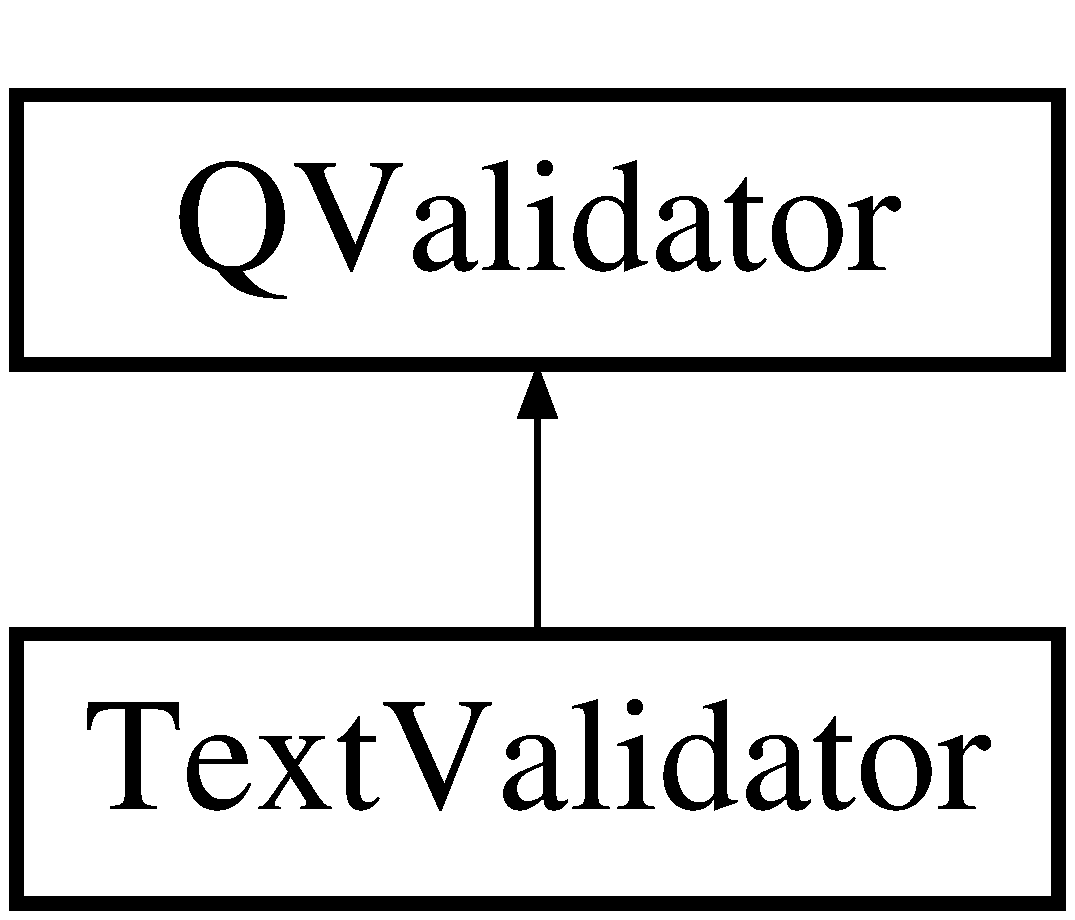
\includegraphics[height=2.000000cm]{class_text_validator}
\end{center}
\end{figure}
\subsection*{Открытые члены}
\begin{DoxyCompactItemize}
\item 
\hyperlink{class_text_validator_a29a44f791c6a0236b562f847deefa527}{Text\+Validator} (Q\+Object $\ast$parent=0)
\begin{DoxyCompactList}\small\item\em \hyperlink{class_text_validator_a29a44f791c6a0236b562f847deefa527}{Text\+Validator\+::\+Text\+Validator}. \end{DoxyCompactList}\item 
State \hyperlink{class_text_validator_a42a94c8bf5655196978addd3a2124582}{validate} (Q\+String \&, int \&) const 
\begin{DoxyCompactList}\small\item\em \hyperlink{class_text_validator_a42a94c8bf5655196978addd3a2124582}{Text\+Validator\+::validate}. \end{DoxyCompactList}\end{DoxyCompactItemize}


\subsection{Конструктор(ы)}
\index{Text\+Validator@{Text\+Validator}!Text\+Validator@{Text\+Validator}}
\index{Text\+Validator@{Text\+Validator}!Text\+Validator@{Text\+Validator}}
\subsubsection[{\texorpdfstring{Text\+Validator(\+Q\+Object $\ast$parent=0)}{TextValidator(QObject *parent=0)}}]{\setlength{\rightskip}{0pt plus 5cm}Text\+Validator\+::\+Text\+Validator (
\begin{DoxyParamCaption}
\item[{Q\+Object $\ast$}]{parent = {\ttfamily 0}}
\end{DoxyParamCaption}
)}\hypertarget{class_text_validator_a29a44f791c6a0236b562f847deefa527}{}\label{class_text_validator_a29a44f791c6a0236b562f847deefa527}


\hyperlink{class_text_validator_a29a44f791c6a0236b562f847deefa527}{Text\+Validator\+::\+Text\+Validator}. 


\begin{DoxyParams}{Аргументы}
{\em parent} & \\
\hline
\end{DoxyParams}


\subsection{Методы}
\index{Text\+Validator@{Text\+Validator}!validate@{validate}}
\index{validate@{validate}!Text\+Validator@{Text\+Validator}}
\subsubsection[{\texorpdfstring{validate(\+Q\+String \&, int \&) const }{validate(QString &, int &) const }}]{\setlength{\rightskip}{0pt plus 5cm}Q\+Validator\+::\+State Text\+Validator\+::validate (
\begin{DoxyParamCaption}
\item[{Q\+String \&}]{text, }
\item[{int \&}]{pos}
\end{DoxyParamCaption}
) const}\hypertarget{class_text_validator_a42a94c8bf5655196978addd3a2124582}{}\label{class_text_validator_a42a94c8bf5655196978addd3a2124582}


\hyperlink{class_text_validator_a42a94c8bf5655196978addd3a2124582}{Text\+Validator\+::validate}. 


\begin{DoxyParams}{Аргументы}
{\em text} & \\
\hline
{\em pos} & \\
\hline
\end{DoxyParams}
\begin{DoxyReturn}{Возвращает}

\end{DoxyReturn}


Объявления и описания членов классов находятся в файлах\+:\begin{DoxyCompactItemize}
\item 
customvalidator.\+h\item 
customvalidator.\+cpp\end{DoxyCompactItemize}

\hypertarget{class_word_validator}{}\section{Класс Word\+Validator}
\label{class_word_validator}\index{Word\+Validator@{Word\+Validator}}
Граф наследования\+:Word\+Validator\+:\begin{figure}[H]
\begin{center}
\leavevmode
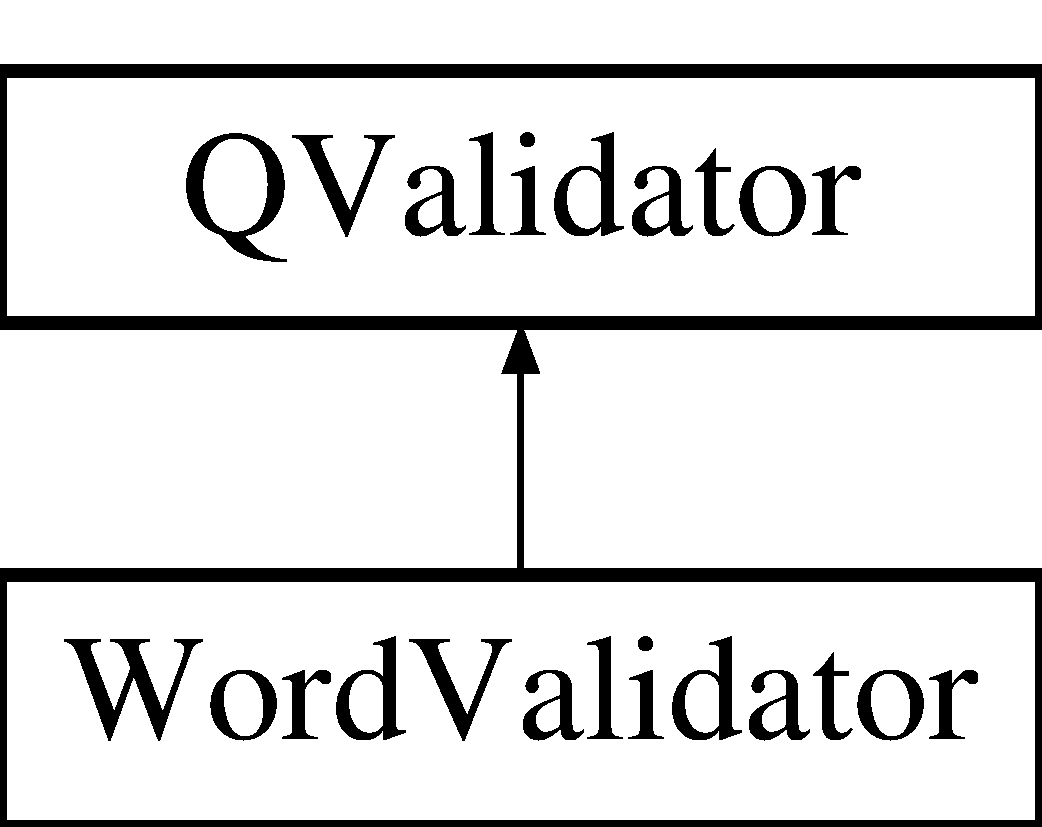
\includegraphics[height=2.000000cm]{class_word_validator}
\end{center}
\end{figure}
\subsection*{Открытые члены}
\begin{DoxyCompactItemize}
\item 
\hyperlink{class_word_validator_a055e67ae8b4af520d431d6e2fadea006}{Word\+Validator} (Q\+Object $\ast$parent=0)
\begin{DoxyCompactList}\small\item\em \hyperlink{class_word_validator_a055e67ae8b4af520d431d6e2fadea006}{Word\+Validator\+::\+Word\+Validator}. \end{DoxyCompactList}\item 
State \hyperlink{class_word_validator_afa4709ee674801c25513b588c8a3d0c1}{validate} (Q\+String \&, int \&) const 
\begin{DoxyCompactList}\small\item\em \hyperlink{class_word_validator_afa4709ee674801c25513b588c8a3d0c1}{Word\+Validator\+::validate}. \end{DoxyCompactList}\end{DoxyCompactItemize}


\subsection{Конструктор(ы)}
\index{Word\+Validator@{Word\+Validator}!Word\+Validator@{Word\+Validator}}
\index{Word\+Validator@{Word\+Validator}!Word\+Validator@{Word\+Validator}}
\subsubsection[{\texorpdfstring{Word\+Validator(\+Q\+Object $\ast$parent=0)}{WordValidator(QObject *parent=0)}}]{\setlength{\rightskip}{0pt plus 5cm}Word\+Validator\+::\+Word\+Validator (
\begin{DoxyParamCaption}
\item[{Q\+Object $\ast$}]{parent = {\ttfamily 0}}
\end{DoxyParamCaption}
)}\hypertarget{class_word_validator_a055e67ae8b4af520d431d6e2fadea006}{}\label{class_word_validator_a055e67ae8b4af520d431d6e2fadea006}


\hyperlink{class_word_validator_a055e67ae8b4af520d431d6e2fadea006}{Word\+Validator\+::\+Word\+Validator}. 


\begin{DoxyParams}{Аргументы}
{\em parent} & \\
\hline
\end{DoxyParams}


\subsection{Методы}
\index{Word\+Validator@{Word\+Validator}!validate@{validate}}
\index{validate@{validate}!Word\+Validator@{Word\+Validator}}
\subsubsection[{\texorpdfstring{validate(\+Q\+String \&, int \&) const }{validate(QString &, int &) const }}]{\setlength{\rightskip}{0pt plus 5cm}Q\+Validator\+::\+State Word\+Validator\+::validate (
\begin{DoxyParamCaption}
\item[{Q\+String \&}]{text, }
\item[{int \&}]{pos}
\end{DoxyParamCaption}
) const}\hypertarget{class_word_validator_afa4709ee674801c25513b588c8a3d0c1}{}\label{class_word_validator_afa4709ee674801c25513b588c8a3d0c1}


\hyperlink{class_word_validator_afa4709ee674801c25513b588c8a3d0c1}{Word\+Validator\+::validate}. 


\begin{DoxyParams}{Аргументы}
{\em text} & \\
\hline
{\em pos} & \\
\hline
\end{DoxyParams}
\begin{DoxyReturn}{Возвращает}

\end{DoxyReturn}


Объявления и описания членов классов находятся в файлах\+:\begin{DoxyCompactItemize}
\item 
customvalidator.\+h\item 
customvalidator.\+cpp\end{DoxyCompactItemize}

%--- End generated contents ---

%%% Local Variables: 
%%% mode: latex
%%% TeX-master: "rpz"
%%% End: 

%\chapter{Еще картинки}
\label{cha:appendix2}

\begin{figure}
\centering
\caption{Еще одна картинка, ничем не лучше предыдущей. Но надо же как-то заполнить место.}
\end{figure}

%%% Local Variables: 
%%% mode: latex
%%% TeX-master: "rpz"
%%% End: 

%\includedoc{latex/refman}
%\setcounter{page}{\thepage-1}
%% Также можно использовать \Referat, как в оригинале

%\begin{abstract}
	
	\chapter*{РЕФЕРАТ}
	\addcontentsline{toc}{chapter}{РЕФЕРАТ}
	
	Пояснительная записка \begin{NoHyper}{\pageref{LastPage}}\end{NoHyper}~с., 
%	\totchaps~ч., 
	\totfig~рис., \tottab~табл., \totbib~источников.%, \totappend~прил.
	
	 
	
	СЕТЕВОЕ ОБОРУДОВАНИЕ, КОНФИГУРАЦИОННЫЕ ФАЙЛЫ, МАРШРУТИЗАТОРЫ, КОММУТАТОРЫ, CISCO IOS, DHCP, NAT, VLAN, СПИСКИ ДОСТУПА.
	
	Объектом исследования выступает сетевое оборудование компании Cisco Systems
	
	Предметом исследования в дипломной работе являются настройка сетевого оборудование Cisco Systems.
	
	Теоретическая значимость дипломного исследования состоит в развитии и совершенствовании методологии настройки оборудования информационной инфраструктуры предприятия.
	
	Практическая значимость работы определяется тем, что ее результаты позволяют повысить степень эффективности настройки информационной инфраструктуры предприятия и снизить связанные с этим операционные расходы при использовании разработанной системы, направленной на повышение уровня таких аспектов администрирование, как быстрота и легкость обслуживания.
	
	Новизна дипломной работы заключается в разработке и реализации кроссплатформенной модели автоматизации конфигурирования оборудования.
%\end{abstract}

%%% Local Variables: 
%%% mode: latex
%%% TeX-master: "rpz"
%%% End: 
  

\end{document}

%%% Local Variables:
%%% mode: latex
%%% TeX-master: t
%%% End:
